% ****** Start of file apssamp.tex ******
%
%   This file is part of the APS files in the REVTeX 4.1 distribution.
%   Version 4.1r of REVTeX, August 2010
%
%   Copyright (c) 2009, 2010 The American Physical Society.
%
%   See the REVTeX 4 README file for restrictions and more information.
%
% TeX'ing this file requires that you have AMS-LaTeX 2.0 installed
% as well as the rest of the prerequisites for REVTeX 4.1
%
% See the REVTeX 4 README file
% It also requires running BibTeX. The commands are as follows:
%
%  1)  latex apssamp.tex
%  2)  bibtex apssamp
%  3)  latex apssamp.tex
%  4)  latex apssamp.tex
%
\documentclass[%
 reprint,
%superscriptaddress,
%groupedaddress,
%unsortedaddress,
%runinaddress,
%frontmatterverbose,
%preprint,
%showpacs,preprintnumbers,
%nofootinbib,
%nobibnotes,
%bibnotes,
 amsmath,amssymb,
 aps,
%pra,
%prb,
%rmp,
%prstab,
%prstper,
%floatfix,
]{revtex4-1}

\usepackage{graphicx}% Include figure files
\usepackage{dcolumn}% Align table columns on decimal point
\usepackage{bm}% bold math
%\usepackage{hyperref}% add hypertext capabilities
%\usepackage[mathlines]{lineno}% Enable numbering of text and display math
%\linenumbers\relax % Commence numbering lines
\usepackage{mathrsfs}
\usepackage{float}
\usepackage{xcolor}
% \usepackage{sidecap} % add figures that can have text on the side
%\usepackage[showframe,%Uncomment any one of the following lines to test
%%scale=0.7, marginratio={1:1, 2:3}, ignoreall,% default settings
%%text={7in,10in},centering,
%%margin=1.5in,
%%total={6.5in,8.75in}, top=1.2in, left=0.9in, includefoot,
%%height=10in,a5paper,hmargin={3cm,0.8in},
%]{geometry}
% \usepackage[a4paper, total={8in, 10in}]{geometry}
\usepackage[spanish]{babel}
\selectlanguage{spanish}
\usepackage[utf8]{inputenc}
\usepackage{esint}
\usepackage{subcaption} % so can use subfigure
\begin{document}

% \setlength{\itemsep{5em}}

\newcommand{\alfabeto}{\mathcal{A}_X}

\newcommand{\propiedad}{\textcolor{red}{\mathbf{>}}}
\newcommand{\definir}{\color{red}{\textbf{\#}}}
\newcommand{\tema}{\color{red}{\bullet}}
\newcommand{\nota}{\textcolor{red}{\color{red}{\boldsymbol{\sim}}}}
\newcommand{\ejemplo}{\textcolor{red}{\color{red}{\boldsymbol{*}}}}
\newcommand{\demo}{\textcolor{red}{\color{red}{\boldsymbol{\|}}}}

\newcommand*\sepline{%
  \rule[0.7ex]{.5\textwidth}{.5pt}}

%\preprint{APS/123-QED}

\title{Teoría información}% Force line breaks with \\

\maketitle

\textbf{Notación:}

$\nota$: Nota
$,\ \tema$: Tema
$,\ \propiedad$: Propiedad
$,\ \definir$: Definir,

$\ejemplo$: Ejemplo, $\demo$: Demostración

\sepline

\textbf{$\tema$ Matemáticas:}
$$
\begin{aligned}
&\lim _{p \rightarrow 0} p \log (p)=0, \ \sum_{k=0}^{n} a r^{k}=a\left(\frac{1-r^{n+1}}{1-r}\right), \
\sum_{n=1}^{\infty} n r^{n} =\frac{r}{(1-r)^{2}} \\ 
&\sum_{k=k_1}^{k_2} ar^k
=a \frac{r^{k_1} - r^{k_2 + 1}}{1-r}, 
\
\int_{a}^{b} x^n f(kx) dx = \frac{1}{k^{n+1}} \int_{ka}^{kb} u f(u) du
\\
%                 
&\int_{\mathbb{R}} e^{- (ax^2 + bx + c )} = \sqrt{\frac{\pi}{a}} e^{ ( \frac{b^2}{4a} - c )}
,\
\delta (p -p') = \frac{1}{2\pi} \int_{\mathbb{R}} e^{i(p-p')\xi} d\xi
\end{aligned}
$$

\textbf{$\propiedad$ La truca para estas }
$$
\begin{aligned}
%
&I = \int _ { a } ^ { b } x ^ { n } e ^ { \pm \alpha x } d x
, \ 
{ \partial _ { \alpha } e ^ { \pm \alpha x } = ( \pm 1 ) x e ^ { t \alpha x } } , \ { \partial _ { \alpha } ^ { n } e ^ { \pm \alpha x } = ( \pm 1 ) ^ { n } x ^ { n } e ^ { \pm \alpha x } } \\
% 
& I = ( \pm 1 ) ^ { n } \partial _ { \alpha } ^ { n } \int _ { a } ^ { b } e ^ { \pm \alpha x } d x \Rightarrow I = \left. ( \pm 1 ) ^ { n+1 } \partial _ { \alpha } ^ { n } { \frac{e ^ { \pm \alpha x }}{\alpha} } \right| ^{ b }_ { a } \\
% 
&\Rightarrow { \int _ { 0 } ^ { \infty } x ^ { n } e ^ { - x / a } d x = n ! a ^ { n + 1 } } , \ { \int _ { 0 } ^ { \infty } x ^ { 2 n + 1 } e ^ { - x ^ { 2 } / a ^ { 2 } } d x = \frac { n ! } { 2 } a ^ { 2 n + 2 } } \\
% 
& \int _ { 0 } ^ { \infty } x ^ { 2 n } e ^ { - x ^ { 2 } / a ^ { 2 } } d x =  (-1)^n \sqrt { \pi } \partial_\alpha^n (\alpha^{-1/2}) \\
% 
&
\textbf{Otra:}  \int_0 ^t e^{\alpha \varepsilon} d \varepsilon = \frac{1}{\alpha} (e^{\alpha t} - 1)\\
%
&
^\textbf{Distr.}
_\textbf{cauchy}
f\left(x ; x_{0}, \gamma\right)=\frac{1}{\pi \gamma\left[1+\left(\frac{x-x_{0}}{\gamma}\right)^{2}\right]}
,\
^\text{$x_0$: ancho}
_\text{$g$: ancho a mitad de altura}
\end{aligned}
$$

\textbf{$\tema$ Probabilidades:} $A: \text{event }A, \quad \bar{A}: \text{Not event }A $
\begin{itemize}
  \item[$\propiedad$] $P(A)+P(\bar{A})=1$
  \item[$\propiedad$] $P(A \cup B)=P(A)+P(B)-P(A \cap B)$ (A or B)
  \item[$\propiedad$] $P(A, B)=P(A \cap B)=P(A \mid B) P(B)$ (A and B)
  \item[$\propiedad$] $P\left(E_{i} \mid E\right)=\frac{P\left(E_{i}\right) P\left(E \mid E_{i}\right)}{\sum_{j=1}^{k} P\left(E \mid E_{j}\right) P\left(E_{j}\right)}$ (Baye's Formula)
  \item[$\propiedad$] $P(A \mid B)=P(A)$ (Independent Trials)

  \item[$\propiedad$] 
  $E[X] =\langle x \rangle = \int_\mathbb{R} x p(x) dx$ (continuo)

  $E[X] =\langle x \rangle = \sum_{i=1}^k x_i p_i$ (discreto)
  
  \item[$\propiedad$] 
  $\operatorname{Var}(X) =E\left[(X-E[X])^{2}\right]$

  $
  \begin{aligned}
  \operatorname{Var}(X) &=E\left[X^{2}-2 X E[X]+E[X]^{2}\right] \\
  &=E\left[X^{2}\right] - 2 E[X E[X] ] +E[X]^{2} \\
  &=E\left[X^{2}\right]-E[X]^{2}
  \end{aligned}
  $

  \item[$\propiedad$] Probability of one of $k$ mutually exclusive events
  
  $
  P=P\left(E_{1}\right)+P\left(E_{2}\right)+\ldots+P\left(E_{k}\right)
  $
  
  \item[$\propiedad$]
  Total Probability, $k$ mutually exclusive events:
  $$
  \begin{aligned}
    P(E)&=P\left(E \mid E_{1}\right) P\left(E_{1}\right)+\ldots+P\left(E \mid E_{k}\right) P\left(E_{k}\right)\\
    &=\sum_{i=1}^{k} P\left(E \mid E_{i}\right) P\left(E_{i}\right) 
  \end{aligned}
  $$

  \item[$\propiedad$] Variable change, prob. density functions:
  $$
  g(\vec{y}) = f(\vec{x}) \left|
    {
    \det
  \left(\frac{d\vec{x}}{d\vec{y}}\right)
  }
  \right|
  $$
\end{itemize}


\section{Introducción}

\textbf{$\tema$ Notación:}

\begin{itemize}
  \item[] $\mathcal{A}_X : \text{Alfabeto de la variable aleatoria $X$}$
  \item[] $p_i: \text{Probabilidades}$
  \item[] $l_i: ^\text{\# de preguntas necesarias para }_\text{llegar al elemento $i$ del alfabeto}$
  \item[] $H: \text{Entropía} $
  \item[] $C(x):$ palabra clave asociada a $x .$
  \item[] $\ell(x):$ longitud de $C(x)$, medida en dígitos. 
\end{itemize}

\textbf{$\definir$ Num. medio de preguntas en pie de igualdad:}
$$
\left\langle\begin{array}{c}
\# \text { preguntas en pie de igualdad} \\
\text { bien elegidas }
\end{array}\right\rangle=\sum_{i} p_{i} \ell_{i}
$$
Usando: $
p_{i}=D^{-\ell_{i}}
\Leftrightarrow
\ell_{i}=-\log _{D} p_{i}
$
$$
\text{Se tiene: }
\left\langle\begin{array}{c}
\# \text { preguntas } \\
\text { bien elegidas }
\end{array}\right\rangle=-\sum_{i} p_{i} \log _{D} p_{i}
$$

\textbf{$\definir$ Entropía:}
$$
H=-\sum_{i} p_{i} \log _{D} p_{i}
$$

\textbf{$\propiedad$ Conversión de unidades:}
$$
H_{D}=-\sum p_{i} \log _{D} p_{i}=-\sum p_{i} \frac{\log _{D^{\prime}}\left(p_{i}\right)}{\log _{D^{\prime}}(D)}=\frac{1}{\log _{D^{\prime}}(D)} H_{D^{\prime}}
$$

\textbf{$\tema$ Propiedades de $H$:}
\begin{enumerate}
  \item[$\propiedad$] Anidación: 
  Si $Y=f(X)$, $\mathcal{C}(y) \subset \mathcal{A}_{X}$ contiene a todo $x:x \stackrel{f}{\rightarrow} y$ 
  % mapeado en $y$ por $f$, 
  $\Rightarrow$
  $$
  H(X)=H(Y)-\sum_{y} p(y) \sum_{x \in C(y)} p(x \mid y) \log [p(x \mid y)
  $$
  \item[$\propiedad$] Cotas y sus implicaciones:
  $$
  \underbrace{0}_{\text{Determinista}} \leq H(X)
  \leq \underbrace{\log|A_X|}_{\text{Uniforme}}
  $$
\end{enumerate}

\textbf{$\tema$ Caso bivariado:}
Con $\mathbf{X}=\left(X_{1}, X_{2}\right)$ variable aleatoria bivariada, $\mathbf{X} \in \mathcal{A}_{X_{1}}\times\mathcal{A}_{X_{2}}$ con prob. conjunta $p\left(x_{1}, x_{2}\right)$

\textbf{$\definir$ Entropía conjunta:}
$$
H\left(X_{1}, X_{2}\right)=-\sum_{x_{1}} \sum_{x_{2}} p\left(x_{1}, x_{2}\right) \log _{D}\left[p\left(x_{1}, x_{2}\right)\right]
$$

\textbf{$\definir$ Entropías marginales(una a una): }
$$
\begin{aligned}
H\left(X_{1}\right)&=-\sum_{x_{1}} p\left(x_{1}\right) \log _{D}\left[p\left(x_{1}\right)\right] \\
H\left(X_{2}\right)&=-\sum_{x_{2}} p\left(x_{2}\right) \log _{D}\left[p\left(x_{2}\right)\right] \\
&\text{distr. marginales } \\
p\left(x_{1}\right)&=\sum_{x_{2}} p\left(x_{1}, x_{2}\right), \
p\left(x_{2}\right)=\sum_{x_{1}} p\left(x_{1}, x_{2}\right)
\end{aligned}
$$

\textbf{$\definir$ Entropía condicional:}
$$
\begin{aligned}
H\left(X_{1} \mid X_{2}\right)=-\sum_{x_{2}} p\left(x_{2}\right) \sum_{x_{1}} p\left(x_{1} \mid x_{2}\right) \log _{D}\left[p\left(x_{1} \mid x_{2}\right)\right] \\
H\left(X_{2} \mid X_{1}\right)=-\sum_{x_{1}} p\left(x_{1}\right) \sum_{x_{2}} p\left(x_{2} \mid x_{1}\right) \log _{D}\left[p\left(x_{2} \mid x_{1}\right)\right]
\end{aligned}
$$

\textbf{$\propiedad$ Regla de la cadena: }
$$
\begin{aligned}
  H(X, Y) &= H(X)+H(Y \mid X) \\ 
        &= H(Y)+H(X \mid Y)
\end{aligned}
$$
$$
\left\|
\begin{aligned}
H(X, Y) &=-\sum_{x} \sum_{y} p(x, y) \log [p(x, y)] \\
&=-\sum_{x} \sum_{y} p(x) p(y \mid x) \log [p(x) p(y \mid x)] \\
&=-\sum_{x} p(x) \sum_{y} p(y \mid x)\{\log [p(x)]+\log [p(y \mid x)]\} \\
&=-\sum_{x} p(x) \log [p(x)] \underbrace{\sum_{y} p(y \mid x)}_{1}  \\
& \quad  - \sum_{x} p(x) \sum_{y} p(y \mid x) \log [p(y \mid x)] \\
&=H(X)+H(Y \mid X)
\end{aligned}
\right.
$$

\textbf{$\propiedad$ Regla de la cadena multivariable: }
$$
H\left(X_{1}, X_{2}, \ldots, X_{n}\right)=\sum_{i=1}^{n} H\left(X_{i} \mid X_{i-1}, \ldots, X_{1}\right)
$$


\textbf{$\propiedad$ Cotas $H$ condicional:}
$$
\underbrace{0}_{\text{determinista}} \leq H(X \mid Y) \leq \underbrace{H(X)}_{\text{Independientes}}
\leq \underbrace{\log|A_X|}_{\text{Uniforme}}
$$

\textbf{$\propiedad$ Cotas $H$ multivariable:}
$$
H\left(X_{1}, X_{2}, \ldots, X_{N}\right) \leq \sum_{i} H\left(X_{i}\right)
$$

\textbf{$\propiedad$} $H(X|X) = H(X)$

\textbf{$\propiedad$ Condición de independencia:} 
$$
\begin{aligned}
  X, Y \text{ son independientes} & \Leftrightarrow H(X \mid Y)=H(X) \\
  X, Y \text{ son independientes} & \Leftrightarrow H(Y \mid X)=H(Y) \\
  X, Y \text{ son independientes} & \Leftrightarrow H(X, Y) = H(X)+H(Y)
\end{aligned}
$$

\textbf{$\propiedad$} 
$H(X, Y \mid Z)=H(X \mid Z) + H(Y \mid X,Z)$

\section{Clase 2:}

\textbf{$\definir$ Función convexa:} 
$f(x)$ es convexa en el intervalo $[a, b]$ $\Leftrightarrow \forall x_{1}, x_{2} \in [a, b]$, $\forall \lambda \in[0,1]$:
$$
\underbrace{f\left[\lambda x_{1}+(1-\lambda) x_{2}\right]}_{\text {Gráfico de $f$ en } x \in (x_1,x_2)} \leq \underbrace{\lambda f\left(x_{1}\right)+(1-\lambda) f\left(x_{2}\right)}_{\text {Cuerda en } x \in (x_1,x_2)}
$$

\textbf{$\definir$ Estrictamente convexa:} 
La función es convexa y únicamente en los extremos se cumple la igualdad.

\textbf{$\propiedad$} Si $f''>0(f''>0)$ en un intervalo $I$ $\Rightarrow$ es estrictamente convexa (cóncava) en $I$.

\textbf{$\propiedad$ Desigualdad de Jansen:} 
Si $f: \mathbb{R} \rightarrow \mathbb{R}$ es convexa, y $X$ es una variable aleatoria$\Rightarrow$
$$
\langle f(X)\rangle \geq f(\langle X\rangle), \quad
\forall \text{ distribución } p(x)
$$

\textbf{$\nota$} 
Si $f$ es estrictamente convexa, $\langle f(X)\rangle = f(\langle X\rangle)$
$\Leftrightarrow$ $X$ es determinista.

\textbf{$\propiedad$ Desigualdad de la suma de logaritmos:} Dados $a_{1}, \ldots, a_{n} \in \mathbb{R}^+_0$, $b_{1}, \ldots, b_{n} \in \mathbb{R}^+$
$$
\sum_{i=1}^{n} a_{i} \log \left(\frac{a_{i}}{b_{i}}\right) \geq\left(\sum_{i=1}^{n} a_{i}\right) \log \left(\frac{\sum_{j=1}^{n} a_{j}}{\sum_{k=1}^{n} b_{k}}\right)
$$

\textbf{$\nota$} 
$(\geq)$ se vuelve (=) $\Leftrightarrow$ $\frac{a_{i}}{b_{i}} = \text{cte.}$ (no depende de $i$).

\textbf{$\definir$ Divergencia de Kullback-Leibler:}
Dadas $p\left(x_{i}\right)$, $q\left(x_{i}\right)$ distr. de prob. con $x_i \in A_X, \forall i$:
$$
D_{\mathrm{KL}}(p \| q)=\sum_{i} p\left(x_{i}\right) \log \left[\frac{p\left(x_{i}\right)}{q\left(x_{i}\right)}\right]
$$

\textbf{$\propiedad$ Justificando en término de \# preguntas sobrantes:}
$$
\left\langle
\#
^\text {preguntas} _\text{sobrantes}
\right\rangle
=
\left\langle
\#
^\text {preguntas requeridas}
_\text {con la estrategia de q}
\right\rangle
-
\left\langle
\# 
^\text { preguntas requeridas }
_\text { con la estrategia de p}
\right\rangle
$$
$ \text{Además, }
\langle
\# 
^\text { preguntas requeridas }
_\text { con la estrategia de q}
\rangle 
=
\sum_{i} \underbrace{p\left(x_{i}\right)}$

$\qquad \qquad \qquad \qquad \qquad =-\sum_{i} p\left(x_{i}\right) \log _{D}\left[q\left(x_{i}\right)\right]$

\textbf{$\tema$ Propiedades $D_{KL}$: }

\begin{enumerate}
  \item[$\propiedad$] $\underbrace{0}_{p=q} \leq D_{\mathrm{KL}}(p \| q)$
  \item[$\propiedad$] $D_{\mathrm{KL}}$ es convexa

  \item[-] $\exists$ (muchos) casos en los que:
  \begin{itemize}
    \item[$\propiedad$] $D_{\mathrm{KL}}(p \| q) \neq D_{\mathrm{KL}}(q \| p)$ (Asimetría) 
    \item[$\propiedad$] $D_{\mathrm{KL}}(p \| q)+D_{\mathrm{KL}}(q \| r)<D_{\mathrm{KL}}(r \| p)$ (Desigualdad triangular)
    \item[$\propiedad$] $D_{\mathrm{KL}}$ diverge ($=\infty$)
  \end{itemize}
\end{enumerate}

\textbf{$\definir$ Información mutua:} 
Con variables aleatorias $X$,$Y$ con distr. conjunta $p(x, y)$, la info.
mutua $I(X ; Y)$ entre ellas se define como
$$
\begin{aligned}
I(X ; Y) &=H(Y)-H(Y \mid X) \\
&=H(X)-H(X \mid Y) \\
&=H(X)+H(Y)-H(X, Y) \\
&=D_{\mathrm{KL}}[p(x, y) \| p(x) p(y)] \\
&=\sum_{x \in\{0,1\}} \sum_{y \in\{0,1\}} p(x, y) \log \left[\frac{p(x, y)}{p(x) p(y)}\right]
\end{aligned}
$$

\textbf{$\nota$} Las dos variables se separan por ; Por ejemplo, 
$$
\begin{aligned}
  I\left(X_{1}, X_{2} ; Y_{1}, Y_{2}, Y_{3}\right) &= H\left(X_{1}, X_{2}\right) \\
  & - H\left(X_{1}, X_{2} \mid Y_{1}, Y_{2}, Y_{3}\right)
\end{aligned}
$$

\textbf{$\definir$ Información mutua condicionada:}
$$
\begin{aligned}
I(X ; Y \mid Z) &=H(X \mid Z)-H(X \mid Y, Z) \\
&=H(Y \mid Z)-H(Y \mid X, Z) \\
&=H(X \mid Z)+H(Y \mid Z)-H(X, Y \mid Z) \\
&=\sum_{z} p(z) D_{\mathrm{KL}}[p(x, y \mid z) \| p(x \mid z) p(y \mid z)]
\end{aligned}
$$
donde $X, Y, Z$ son variables aleatorias.

\textbf{$\definir$ $I$ condicionada multivariada:} 
$$
I\left(X_{1}, X_{2}, \ldots, X_{n} ; Y\right)=\sum_{i=1}^{n} I\left(X_{i} ; Y \mid X_{i-1}, X_{i-2}, \ldots, X_{1}\right)
$$
$$
\left\|
\begin{aligned}
I & \left(X_{1}, X_{2}, \ldots, X_{n} ; Y\right) = \\
\quad &=H\left(X_{1}, X_{2}, \ldots, X_{n}\right)-H\left(X_{1}, X_{2}, \ldots, X_{n} \mid Y\right) \\
\quad &=\sum_{i=1}^{n} H\left(X_{i} \mid X_{i-1}, \ldots, X_{1}\right)\\
&-\sum_{i=1}^{n} H\left(X_{i} \mid X_{i-1}, \ldots, X_{1}, Y\right) \\
\quad &=\sum_{i=1}^{n} I\left(X_{i} ; Y \mid X_{1}, X_{2}, \ldots, X_{i-1}\right)
\end{aligned}
\right.
$$

\textbf{$\propiedad$} $ I(X ; Y, Z)=I(X ; Y)+I(X ; Z \mid Y) $

\textbf{$\tema$ Propiedades de $I$ mutua: }

\begin{enumerate}
  \item[$\propiedad$] $I(X)$(y $H(X)$)no depende de $X$, solo de sus prob.
  \item[$\propiedad$] $ I(X ; X)=H(X) $ (viene de $H(X \mid X)=0$)
  \item[$\propiedad$] $ I(X ; Y)=I(Y ; X) $ (simetría)
  \item[$\propiedad$]   
  $Y=f(X), f \ ^\text{funcion}_\text{inyectiva} \Rightarrow I(X ; Y)=H(X)=H(Y)$
  \item[$\propiedad$] Variables aleatorias $X, Y, Z=f(Y)$ 
  
  $\Rightarrow$
  $I(X ; Y) \geq I(X ; Z)$
\end{enumerate}


\textbf{$\propiedad$ Cota $I$ mutua:} 
$$
\begin{aligned}
  \underbrace{0}_\text{independiente} \leq I(X ; Y) & \leq \underbrace{\min [H(X), H(Y)]}_\text{determinista} \\
  \underbrace{0}_\text{independiente} \leq I(X ; Y) & \leq \underbrace{\min \left[\log \left| \mathcal{A}_{X} \right|, \log \left|\mathcal{A}_{Y}\right| \right]}_\text{uniforme}
\end{aligned}
$$

\textbf{$\definir$ Estadística suficiente:} 
Un mapeo $z=f(y)$ es una estadística suficiente $\Leftrightarrow$ $I(X ; Y)=I(X ; Z)$.

\section{Clase 3:}

\textbf{$\definir$ Convergencia en probabilidad:} 
Una secuencia de variables aleatorias $\left(X_{1}, X_{2}, \ldots\right)$ $\rightarrow$ $x_{0}$ en prob. $\Leftrightarrow$ $\forall \varepsilon>0: \operatorname{Pr}\left[\left|X_{n}-x_{0}\right|>\varepsilon\right] \rightarrow 0$ cuando $n \rightarrow \infty .$ Aquí $\operatorname{Pr}\left[\left|X_{n}-x_{0}\right|>\varepsilon\right] \rightarrow 0$ involucra un límite normal, ya que la prob. no es una variable aleatoria. 
$$\text{Es decir,}
\int_{x_{n} :\left|x_{n}-x_{0}\right|>\varepsilon} P(x) \mathrm{d} x \rightarrow 0
$$

\textbf{$\definir$ Convergencia en valor cuadratico medio:}
Una secuencia de variables aleatorias $\left(X_{1}, X_{2}, \ldots\right)$ $\rightarrow$ $x_{0}$ en valor cuad. medio $\Leftrightarrow$ $\left\langle\left(X_{n}-x_{0}\right)^{2}\right\rangle$ $\rightarrow 0$ cuando $n \rightarrow \infty .$ 
$$ \text{Es decir,}
\int_{-\infty}^{+\infty} P\left(x_{n}\right)\left(x_{n}-x_{0}\right)^{2} \mathrm{~d} x_{n} \rightarrow 0
$$

\textbf{$\definir$ Convergencia con probabilidad 1:}
Una secuencia de variables aleatorias $\left(X_{1}, X_{2}, \ldots\right)$ $\rightarrow$  $x_{0}$ con prob. 1, o casi con seguridad $\Leftrightarrow$  $\operatorname{Pr}\left(X_{n}=x_{0}\right) \rightarrow 1,$ cuando $n \rightarrow \infty$. 
$$ \text{Es decir,}
\lim _{\delta \rightarrow 0} \int_{-\infty}^{+\infty} P\left(x_{n}\right) \frac{e^{-\left(x_{n}-x_{0}\right)^{2} / 2 S^{2}}}{\sqrt{2 \pi \delta^{2}}} \rightarrow 1
$$
la prob. $\operatorname{Pr}\left(X_{n}=x_{0}\right)$ es la integral de una $\delta$ Dirac, y usamos una
aprox. cualquiera de la $\delta$. Lo importante es que $\delta \rightarrow 0$ debe tomarse antes que el otro limite. 

\textbf{$\propiedad$ Niveles de exigencia:}
$$
\begin{aligned}
  \text{en prob.} < 
  \text{en valor cuadr. medio} < 
  \text{con prob. 1}
\end{aligned}
$$

\textbf{$\definir$ iid:} independiente(s) e idénticamente distribuida(s).

\textbf{$\propiedad$ La ley de los grandes números:} 
Dada una secuencia de variables aleatorias $X_{1}, X_{2}, \ldots, X_{n}$ \textbf{iid}s con prob. $p(x),$ donde $x \in\left\{a_{1}, \ldots, a_{k}\right\},$ la ley establece que:
$$
\begin{aligned}
  &\frac{1}{n} \sum_{i=1}^{n} f\left(X_{i}\right) 
  \rightarrow
  \sum_{k=1}^{k} p\left(a_{k}\right) f\left(a_{k}\right) \text{en prob.} \text{(Forma débil)}\\
  &\qquad \text{Forma débil}
  \text{(en prob.)} 
  , 
  \text{Forma fuerte}
  \text{(en prob. 1.)} 
\end{aligned}
$$
La primera $\sum$ es un promedio de una función $f$ evaluada en una muestra particular, es
una variable aleatoria. La segunda $\sum$ es el valor medio de $f$ aplicada a los elementos del
alfabeto, no es una variable aleatoria. 

\textbf{$\propiedad$ Teorema de equipartición asintótica:}
Si $X_{1}, X_{2}, \ldots, X_{n}$ son variables aleatorias \textbf{iid} con prob.
$p(x)$, $\Rightarrow$ la variable aleatoria
$$
-\frac{1}{n} \log p\left(X_{1}, \ldots, X_{n}\right) \rightarrow H(X) \text { en probabilidad. }
$$
$-\frac{1}{n} \log p\left(X_{1}, \ldots, X_{n}\right)$ es una variable aleatoria, ya que $p$(determinista) está evaluada en una variable aleatoria. $H(X)$, en
cambio, es determinista.


\textbf{$\definir$ Conjunto típico:} 
El conjunto típico $\mathcal{A}_{\varepsilon}^{(n)}$ con respecto a $p(x)$ es el conjunto de secuencias $\left(x_{1}, \ldots, x_{n}\right) \in\left(\mathcal{A}_{X}\right)^{n}$
que cumplen
$$
2^{-n[H(X)+\varepsilon]} \leq p\left(x_{1}, \ldots, x_{n}\right) \leq 2^{-n[H(X)-\varepsilon]}
$$

\textbf{$\nota$} 
$H(X)$ no depende de la cadena, $X$ es el nombre de la variable aleatoria. La condición para pertenecer al $\mathcal{A}_{\varepsilon}^{(n)}$ es una condición sobre la prob. de la cadena.

\textbf{$\nota$ PUEDE NO SER 2} 
puede ser otra base, $e,3$ o lo que convenga para el problema (unidades de info.).

\textbf{$\tema$ Propiedades conjunto típico$\mathcal{A}_{\varepsilon}^{(n)}$:}

\begin{enumerate}
  \item[$\propiedad$] Si una cadena $\in\mathcal{A}_{\varepsilon}^{(n)}$, el logaritmo de su prob. está muy cercana a $[-n H(X)]$. Esto es, 
  $$
  \begin{aligned}
    \left(x_{1}, \ldots, x_{n}\right) & \in \mathcal{A}_{\varepsilon}^{(n)} \Leftrightarrow\\
    H(X)-\varepsilon \leq-\frac{1}{n} & \log _{2} p\left(x_{1}, \ldots, x_{n}\right) \leq H(X)+\varepsilon
  \end{aligned}$$
  
  \item[$\propiedad$] La prob. de muestrear una cadena del conjunto típico se hace tan grande como querramos,
  aumentando la longitud de las cadenas. Esto es,
  $$
  \forall \delta>0, \exists n_{0} \in \mathbb{N} / \forall n>n_{0}, \operatorname{Prob}\left[\left(X_{1}, \ldots, X_{n}\right) \in \mathcal{A}_{e}^{(n)}\right]>1-\delta
  $$
  \item[$\propiedad$] Cota a cardinalidad del conjunto típico:
  $$
  \underbrace{(1-\varepsilon) 2^{n[H(X)-\varepsilon]}}_{\forall \varepsilon>0, \exists n_{0} \in \mathbb{N} : \forall n>n_{0}(n \text{ big enough})}
  \leq
  \left|\mathcal{A}_{\varepsilon}^{(n)}\right| 
  \leq 
  \underbrace{2^{n[H(X)+\varepsilon]}}_{siempre}
  $$
\end{enumerate}

\textbf{$\propiedad$ Teorema de codificación de una fuente:}
Una secuencia de $n$ variables aleatorias \textbf{iid}, cada una con entropía $H,$ puede representarse por $n(H+\varepsilon)$
dígitos, con $\varepsilon$ tan chico como queramos, y con prob. de pérdida de info. también tan chica
como queramos, si $n$ es lo suficientemente grande. Si se representan con menos de $n H$ dígitos $\Rightarrow$
seguro que hay pérdida de info. (no infinitesimal).

\section{Clase 4:}

\textbf{$\definir$ Código fuente:} 
Dada una variable aleatoria $X$ con alfabeto $\mathcal{A}_{X}, \mathrm{y}$ un alfabeto $\mathcal{A}_{Y}=$
$\{0,1, \ldots, D-1\},$ un código fuente para $X$ es un mapeo $C: \mathcal{A}_{X} \rightarrow$ $^\text{cadenas finitas}
_\text{de elementos de}$
$\mathcal{A}_{Y},$ que también suelen llamarse ``cadenas $D$ -arias finitas".

\textbf{$\definir$ Código fuente no singular:} 
Un código fuente es no singular si es invertible(como las matrices). Es decir, si símbolos distintos del alfabeto son mapeados en secuencias $D$-arias distintas.

\textbf{$\ejemplo$ Ejemplo no singular y singular:}
Los código $C_{0}$, $C_{1}$ mapean el alfabeto $\{a, b, c, d\}$ en tiras compuestas de \{0,1\} , tal que
% El código $C_{0}$ mapea el alfabeto $\{a, b, c, d\}$ en tiras compuestas de \{0,1\} , tal que
% $$
% \begin{array}{c|c|c}
% x & C_{0}(x) & \ell(x) \\
% \hline a & 1000 & 4 \\
% b & 0100 & 4 \\
% c & 0010 & 4 \\
% d & 0001 & 4
% \end{array}
% $$
% \textbf{$\ejemplo$ Ejemplo singular:} 
% El código $C_{1}$ mapea el alfabeto $\{a, b, c, d\}$ en tiras compuestas de \{0,1\} , tal que
% $$\begin{array}{c|c|c}
% x & C_{1}(x) & \ell(x) \\
% \hline a & 10 & 2 \\
% b & 0 & 1 \\
% c & 10 & 2 \\
% d & 010 & 3
% \end{array}
% $$
$$
\text{No singular:}
\begin{array}{c|c|c}
x & C_{0}(x) & \ell(x) \\
\hline a & 1000 & 4 \\
b & 0100 & 4 \\
c & 0010 & 4 \\
d & 0001 & 4
\end{array}\quad 
\text{Singular:}
\begin{array}{c|c|c}
x & C_{1}(x) & \ell(x) \\
\hline a & 10 & 2 \\
b & 0 & 1 \\
c & 10 & 2 \\
d & 010 & 3
\end{array}
$$

\textbf{$\definir$ Código fuente extendido:} 
$C^{+}$ es un código fuente extendido para la variable aleatoria $X$ si $C^{+}: \mathcal{A}_{X}^{+} \rightarrow$ $\{0,1, \ldots, D-1\}^{+},$ donde el supra-índice $+$ representa concatenación sin puntuación.

\textbf{$\ejemplo$ Ejemplo, código fuente extendido:} 
$$
C_{0}(a b a c d b)=\underbrace{1000}_{C_{0}(a)} \underbrace{0100}_{C_{0}(b)} \underbrace{1000}_{C_{0}(a)} \underbrace{0010}_{C_{0}(c)} \underbrace{0001}_{C_{0}(d)} \underbrace{0100}_{C_{0}(b)}
$$

\textbf{$\definir$ Código es unívocamente decodificable:}
Código con extension no singular, es decir, si el código extendido es invertible.

\textbf{$\definir$ Prefijo/ autopuntuado/ indice/ instantáneo:} 
Un código fuente donde ninguna palabra clave es prefijo de otra palabra clave.

\textbf{$\propiedad$ Prop.:} 
indices $\subset$ unívocamente decodificables $\subset$ no singulares $\subset$ códigos 

\textbf{$\definir$ Longitud media:} 
La longitud media de un código fuente para la variable aleatoria $X$ con alfabeto $\mathcal{A}_X=\left\{x_{1}, \ldots, x_{k}\right\} \text { con probabilidades } p\left(x_{1}\right), \ldots p(x_{k})$ es:
$$
\qquad L=\sum_{x \in A_{X}} p(x) \ell(x)
$$

\textbf{$\propiedad$ Desigualdad de Kraft:} 
Con alfabetos 
$\mathcal{A}_{X}=\left\{x_{1}, \ldots, x_{M}\right\}$, $\mathcal{A}_{Y}$
$= \{0,1, \ldots, D-1\} $ 
y un conjunto $\left\{\ell_{1}, \ldots, \ell_{M}\right\} \subset \mathbb{Z}^+$, 

$\exists$ código indice $C: \mathcal{A}_{X} \rightarrow$ $^\text{cadenas finitas}
_\text{de elementos de}$
$\mathcal{A}_{Y},$
de longitudes $\left\{\ell_{1}, \ldots, \ell_{M}\right\}$ $\Leftrightarrow$
$$
\sum_{i=1}^{M} D^{-\ell_{i}} \leq 1
$$

\textbf{$\propiedad$ Cota a la longitud media:} 
La longitud media $L$ de un código $D$-ario para una variable aleatoria $X$ cumple: 
$$H_D(X)\leq L $$

\textbf{$\nota$} 
$L = H_D(X)$ $\Leftrightarrow$ 
$\forall x$, $-\log _{D}[p(x)] \in \mathbb{Z}$ (prob. $D$-arias)

Es decir, si todas las prob. son potencias de $\frac{1}{D}$.

\textbf{$\propiedad$ Código Shannon-Elias-Fano:}
Con longitudes
$$
\ell(x)=\left[-\log _{D} p(x)\right]_{+}
$$
donde, $[\cdot]_{+}$ significa redondeo entero \textit{hacia arriba}. Es decir, si las prob. no son $D$-arias $\Rightarrow$ $\exists x \in \mathcal{A}_{X}$ para el cual $-\log _{D}[p(x)] \notin \mathbb{Z}$. !!!! COMPLETAR con el algoritmo

\textbf{$\propiedad$} 
Siempre se puede codificar una variable aleatoria (cualquier prob.) con un código indice tal que
$$
H_{D}(X) \leq L<H_{D}(X)+1
$$

\textbf{$\propiedad$ Código Huffman:} 
\begin{enumerate}
  \item[$\bullet$] Ordenar de mayor a menor(3,2,1) símbolos por su prob.
  \item[$\bullet$] Formar un arbolito $\mathbb{A}$ con nodo donde anoto la prob. de la suma de los menos probables y con hijos los símbolos menos probables, este nodo va en un nivel superior.
  \item[$\bullet$] Repetir los dos pasos anteriores.
  \item[$\bullet$] Completado $\mathbb{A}$ se usa para codificar. Para indicar el símbolo, se baja por $\mathbb{A}$, las ramas, ordenadas de izquierda a derecha (por decir un orden) indican un dígito D-ario que codifica el símbolo. Cada elección de rama al bajar es un dígito distinto, juntando los dígitos al bajar por el $\mathbb{A}$ se tiene el código fuente del símbolo que esta al final de la rama.
\end{enumerate}

\section{Clase 5:}

\textbf{$\propiedad$ Convertir $\zeta \in [0,1] \subset \mathbb{R}$ a base D-aria($\zeta_D$):}
\begin{itemize}
  \item[$\bullet$] Multiplicar $\zeta$ por $D$. La parte entera del resultado es el primer dígito de la expansión en binario.
  \item[$\bullet$] Con $\zeta_D$ hasta orden $r$, tomar la parte decimal del número obtenido en la multiplicación anterior (descartando la parte entera) y multiplicar por $D$. La parte entera del resultado es el dígito $(r+1)$-ésimo de $\zeta_D$.
\end{itemize}

\textbf{$\propiedad$ Transformación de la acumulada:}
Dadas $X, Y$ variables aleatorias definidas en intervalos finitos, con $Y$ uniforme. Se puede convertir $X$ en $Y$ mediante:
$$y = F_X(x) = \int_{-\infty}^x f_X (\xi) d\xi, \quad f_X: \text{Dens. de prob. de } X$$

\textbf{$\definir$ Codificación aritmética:} 

\textbf{La entrada:} 
Tomada como la representación en base $K$ de $\zeta \in [0,1] \subset \mathbb{R}$ la fuente genera una secuencia $z_{1} z_{2} z_{3} \ldots$, con $z_{i} \in\{0,1,2, \ldots, K-1\}$.
$$
\zeta=\sum_{n=1}^{+\infty} z_{n} K^{-n}, \ f_Z (z) \text{ No uniforme}
$$ 

\textbf{La salida:} 
Tomada como la representación en base $D$ de un $F_z(\zeta )$, la fuente genera una secuencia $y_{1} y_{2} y_{3} \ldots$, con $y_{i} \in\{0,1,2, \ldots, D-1\}$.
$$
F_z(\zeta )=\sum_{n=1}^{+\infty} y_{n} D^{-n}, 
\ f_Y (y) \text{ Uniforme}
$$ 

\textbf{$\nota$} Si $\zeta_D$ en un paso le da al palo, vale el valor del palo.
Si $\zeta_{D=2}$ por ej. $\zeta_{D=2}< \frac{1}{2}$ poner 0, $\zeta_{D=2} \geq \frac{1}{2}$ poner 1.


\section{Clase 6:}

\textbf{$\definir$ Canal discreto:} 
$\left(\mathcal{A}_{X}, \mathcal{A}_{Y}, p(y \mid x)\right)$ con el alfabeto de entrada $\mathcal{A}_{X}$, un alfabeto de salida $\mathcal{A}_{Y}$ y un conjunto de prob. de transición $p(y \mid x)$.

\textbf{$\definir$ Canal sin memoria:} 
$$
p\left(y_{1}, \ldots, y_{n} \mid x_{1}, \ldots, x_{n}\right)=\prod_{i=1}^{n} p\left(y_{i} \mid x_{i}\right)
$$

\textbf{$\definir$ Capacidad de un canal(sin memoria):}
$$
\begin{aligned}
C &=\operatorname{max}_{p(x)} I(X ; Y) \\
&=\operatorname{max}_{p(x)} \sum_{x, y} p(x) p(y \mid x) \log \left[\frac{p(y \mid x)}{\sum_{x^{\prime}} p\left(x^{\prime}\right) p\left(y \mid x^{\prime}\right)}\right]
\end{aligned}
$$

\textbf{$\definir$ Optimización de un canal:}
$$\boxed{\text{Fuente}} \stackrel{W}{\rightarrow}
\boxed{\text{Compresor}} \stackrel{Z}{\rightarrow}
\boxed{\text{Codificador}} \stackrel{X}{\rightarrow}
\boxed{\text{Canal}} \stackrel{Y}{\rightarrow}$$

$A_W$ puede no ser equiprobable, $A_Z$ es equiprobable, $A_X$ es tal que optimiza el canal.

\textbf{$\definir$ Canal sin pérdida:} 

$H(X|Y)=0 \equiv I(X;Y)=H(X)$ 

(Puede agregar ruido, pero no hay perdida de info.)

\textbf{$\nota$} 
$H(X|Y)=0 \Leftrightarrow$ $X$ es función de $Y$.
 
\textbf{$\nota$} 
$C =\operatorname{max}_{p(x)} I(X ; Y)= \operatorname{max}_{p(x)}H(X)=\log|A_X|$. Lo cual ocurre para una $p$ uniforme(Donde $H(X)$ es máxima).


\textbf{$\definir$ Canal es determinista:} 

$H(Y|X)=0 \equiv I(X;Y)=H(Y)$ 

(No agrega ruido, aunque puede comprimir dos entradas en una salida (perdiendo info.))

\textbf{$\nota$} 
$H(Y|X)=0 \Leftrightarrow$ $Y$ es función de $X$.
 
\textbf{$\nota$} 
$C =\operatorname{max}_{p(x)} I(X ; Y)= \operatorname{max}_{p(x)}H(Y)=\log|A_Y|$. Lo cual ocurre para una $p$ uniforme(Donde $H(Y)$ es máxima).

\textbf{$\definir$ Canal biyectivo:} 
Es sin perdida y determinista.

\textbf{$\definir$ Canal inutil:} 
$I(X ; Y)=0$

\textbf{$\definir$ Canal simétrico:} 
La matriz $p(y \mid x)$ es tal que:
$$
\text{Todas sus } ^\textbf{FILAS}_\textbf{COLUMNAS} \text{son permutaciones unas de otras.}
$$
$\nota$ En un canal simétrico $
  I(X ; Y)=H(Y)-H(Y \mid X)
  $
  Con, $
  H(Y \mid X)=-\sum_{x} p(x) \sum_{y} p(y \mid x) \log [p(y \mid x)]
  $

\textbf{$\definir$ Capacidad de un canal simétrico:} 
$$C=I(X;Y)\vline_{p(x)\text{uniforme}}$$

\textbf{$\tema$ Propiedades de la capacidad:}
\begin{enumerate}
  \item[$\propiedad$] $C \geq 0$ (ya que $I(X ; Y) \geq 0$)
  \item[$\propiedad$] $C \leq \log \left|\mathcal{A}_{X}\right|$ (ya que $I(X ; Y) \leq \log \left|\mathcal{A}_{X}\right|$)
  \item[$\propiedad$] $C \leq \log \left|\mathcal{A}_{Y}\right|$ (ya que $I(X ; Y) \leq \log \left|\mathcal{A}_{Y}\right|$)
  \item[$\propiedad$] La $p(x)$:$\operatorname{max}_{p(x)} I(X ; Y)$  puede no ser única.
  \item[$\propiedad$] Si $p(x)$: $I(X ; Y)=\log \left|\mathcal{A}_{X}\right|$ o $\log \left|\mathcal{A}_{Y}\right|$ $\Rightarrow$ $C=\log \left|\mathcal{A}_{Y}\right|$ o $\log \left|\mathcal{A}_{Y}\right|$ con $p(x)$.
\end{enumerate}


\textbf{$\propiedad$ Canal binario simétrico:}
$$
\begin{array}{c|cc}
p(y \mid x) & y=0 & y=1 \\
\hline x=0 & 1-f & f \\
x=1 & f & 1-f
\end{array}
\Rightarrow
C=1+f \log f+(1-f) \log (1-f)
$$

\textbf{$\propiedad$ Canal máquina de escribir ruidosa:}

\begin{tabular}{c|ccccc}
  $p(y \mid x)$ & $y=0$ & $y=1$ & $y=2$ & $\ldots$ & $y=N-1$ \\
  \hline$x=0$ & $\frac{1}{2}$ & $\frac{1}{2}$ & 0 & $\ldots$ & 0 \\
  $x=1$ & 0 & $\frac{1}{2}$ & $\frac{1}{2}$ & $\ldots$ & 0 \\
  $\vdots$ & $\vdots$ & $\ddots$ & $\vdots$ & $\vdots$ & $\vdots$ \\
  $x=N-1$ & $\frac{1}{2}$ & 0 & 0 & $\ldots$ & $\frac{1}{2}$
\end{tabular}

En cada fila hay $N-2$ ceros y dos $1 / 2$. Lo mismo para cada columna $\boldsymbol{\therefore}$ el canal es simétrico $\Rightarrow$ para calcular capacidad, basta con calcular la $I$ mutua para $p(x)=\frac{1}{M}$,
$$
\begin{aligned}
I(X ; Y) &=H(Y)-H(Y \mid X) =\log (N)-\log (2) =\log \left(\frac{N}{2}\right)
\end{aligned}
$$
el término $\log (N)$ sale de que las salidas son equiprobables, y el $\log (\frac{1}{2})$ es $H(Y \mid X)$

\section{Clase 7:}

\textbf{$\definir$ Conjunto típico:} 
El conjunto $\tilde{\mathcal{A}}_{(X ; Y) \varepsilon}^{(n)}$ de secuencias $\left(x^{n} ; y^{n}\right)=\left(x_{1}, \ldots, x_{n} ; y_{1}, \ldots, y_{n}\right)$ conjuntamente típicas es

$
\begin{aligned}
  \tilde{\mathcal{A}}_{(X ; Y) \varepsilon}^{(n)} &=
  \left\{  \left(x^{n} ; y^{n}\right) \in \mathcal{A}_{X} \times \mathcal{A}_{Y} \right. \\
          & \left.  /  x^{n} \in \mathcal{A}_{X \varepsilon}^{(n)} \wedge y^{n} \in \mathcal{A}_{Y \varepsilon}^{(n)} \wedge\left(x^{n} ; y^{n}\right) \in \mathcal{A}_{(X ; Y) \varepsilon}^{(n)}\right\} 
\end{aligned}
$

Esta definición incluye tres condiciones:

\begin{itemize}
  \item[$\bullet$] $x^{n} \in \mathcal{A}_{X \varepsilon}^{(n)},$ $\Rightarrow$ $x^{n}$ es típica en $\mathcal{A}_{X}^{n}$ $\Leftrightarrow$
  $$
  \left|-\frac{1}{n} \log \left[p\left(x_{1}, \ldots, x_{n}\right)\right]-H(X)\right| \leq \varepsilon
  $$
  \item[$\bullet$] $y^{n} \in \mathcal{A}_{Y \varepsilon}^{(n)},$ $\Rightarrow$ $y^{n}$ es típica en $\mathcal{A}_{Y}^{n}$ $\Leftrightarrow$
  $$
  \left|-\frac{1}{n} \log \left[p\left(y_{1}, \ldots, y_{n}\right)\right]-H(Y)\right| \leq \varepsilon
  $$
  \item[$\bullet$] $\left(x^{n} ; y^{n}\right) \in \mathcal{A}_{(X ; Y) \varepsilon}^{(n)},$ $\Rightarrow$ $\left(x^{n} ; y^{n}\right)$ es típica en $\left(\mathcal{A}_{X} \times \mathcal{A}_{Y}\right)^{n}$  $\Leftrightarrow$
  $$
  \left|-\frac{1}{n} \log \left[p\left(x_{1}, \ldots, x_{n}, y_{1}, \ldots, y_{n}\right)\right]-H(X, Y)\right| \leq \varepsilon
  $$
  
\end{itemize}

$p\left(x^{n}, y^{n}\right)=p\left(x_{1}, \ldots, x_{n}, y_{1}, \ldots, y_{n}\right)$: prob. conjunta.

$p\left(x^{n}\right)=p\left(x_{1}, \ldots, x_{n}\right)$: prob. marginal de las $x$

$p\left(y^{n}\right)=p\left(y_{1}, \ldots, y_{n}\right)$: prob. marginal de las $y$
$$
\begin{aligned}
p\left(x^{n}\right) &=\int \mathrm{d} y_{1} \cdots \int \mathrm{d} y_{n} p\left(x^{n}, y^{n}\right) \\
p\left(y^{n}\right) &=\int \mathrm{d} x_{1} \cdots \int \mathrm{d} x_{n} p\left(x^{n}, y^{n}\right)
\end{aligned}
$$

\textbf{$\definir$ Canal sin memoria:}
$$
p\left(x^{n} ; y^{n}\right)=\prod_{i=1}^{n} p\left(x_{i}, y_{i}\right)
$$

\textbf{$\nota$ Condición canal sin memoria:} 
Trabajaremos siempre bajo la suposición de que el canal no tiene memoria

\textbf{$\propiedad$ Propiedades de una cadena conjuntamente típica:}

\textbf{$\propiedad$ Probabilidad de muestrear una cadena conjuntamente típica:}
$$
\operatorname{Prob}\left[\left(x^{n} ; y^{n}\right) \in \tilde{\mathcal{A}}_{(X ; Y) \varepsilon}^{(n)}\right] \rightarrow 1, \text { cuando } n \rightarrow+\infty
$$

\textbf{$\propiedad$ Número de cadenas conjuntamente típicas:}
$$
\underbrace{(1-\varepsilon) 2^{n[H(X, Y)-\varepsilon]}}_{\text{si } n \rightarrow \infty } <
\left|\tilde{\mathcal{A}}_{(X, Y) \varepsilon}^{(n)}\right| \leq 2^{n[H(X, Y)+\varepsilon]}$$

\textbf{$\propiedad$ Probabilidad de muestrear por casualidad secuencias conjuntamente típicas:}
Si $x^{n}$ e $y^{n}$ son secuencias de longitud $n$ muestreadas de una distr. de prob. ${q\left(x^{n}, y^{n}\right)}=p\left(x^{n}\right) p\left(y^{n}\right)$, $\Rightarrow$
$$
\underbrace{(1-\varepsilon) 2^{-n[I(X ; Y)+3 \varepsilon]}}_{n \ ^\text{suficientemente} _\text{grande}}
<
\operatorname{Pr}\left[\left(x^{n} ; y^{n}\right) \in \tilde{\mathcal{A}}_{(X, Y)}^{(n)}\right] \leq 2^{-n[I(X ; Y)-3 \epsilon]}
$$

\textbf{$\nota$} 
Esto $\Rightarrow$ si, en vez de muestrear tiras $(x^{n};y^{n})$ usando prob. $p\left(x^{n}, y^{n}\right)$, las muestreamos con $p\left(x^{n}\right)p\left(y^{n}\right)$, es poco probable que $\left(x^{n}; y^{n}\right)$ $\in$ $\tilde{\mathcal{A}}_{(X, Y)}^{(n)}$ ($\approx 2^{-n I(X ; Y)}$).

\textbf{$\definir$ Código:} 
Un código $(\boldsymbol{M}, \boldsymbol{n})$ para un canal discreto $\left[\mathcal{A}_{X}, \mathcal{A}_{Y}, p(y \mid x)\right]$ es (tres cosas):
\begin{enumerate} 
  \item[$\bullet$] Un conjunto de índices $\{1,2, \ldots, M\}$,
  \item[$\bullet$] Función codificadora $f:\{1, \ldots, M\} \rightarrow \mathcal{A}_{X}^{n}$, que a cada mensaje $w \in\{1, \ldots, M\}$ le asigna una cadena de caracteres $f(w) \in \mathcal{A}_{X}^{n} .$ El conjunto de palabras clave $\{f(1), f(2), \ldots, f(M)\}$ se llama libro de códigos,
  \item[$\bullet$] Función decodificadora $g: \mathcal{A}_{Y}^{n} \rightarrow\{1, \ldots, M\}$.
\end{enumerate}

\textbf{$\definir$ Prob. error condicional $\lambda_{i}$:} 
Asociada al mensaje $i$ es la prob. de no decodificar $i$ cuando se transmite $i$. Es decir,
$$
\begin{aligned}
\lambda_{i}=& \operatorname{Prob}\left[g\left(y^{n}\right) \neq i / x^{n}=f(i)\right] \\
=& \sum_{y^{n} / g\left(y^{n}\right) \neq i} \quad \underbrace{
  \operatorname{Prob}\left[y^{n} \mid f(i)\right]}_{
    \substack{
    \text {Probabilidad de recibir } y^{n} \\ \text { cuando se transmite } x^{n}=f(i)
    }
  }
\end{aligned}
$$

\textbf{$\definir$ Máxima probabilidad de error:} 
$$
\text{del código } (M, n) \text{ es }
\lambda_{\operatorname{max}}=\operatorname{max}_{i} \lambda_{i}
$$

\textbf{$\definir$ Probabilidad de error media del código:} 
$$
\bar{\lambda}=\frac{1}{M} \sum_{i=1}^{M} \lambda_{i}
$$

\textbf{$\definir$ Tasa:} 
La tasa $R$ de un código $(M, n)$ es
$$
R=\frac{\log (M)}{n}
$$

\textbf{$\definir$ Tasa realizable:} 
Existe una sucesión de códigos $\left(2^{n R}, n\right)$ cuya máxima prob. de error $\lambda_{\text {mix }}$ tiende a cero cuando $n \rightarrow \infty$.

\textbf{$\propiedad$ Teorema de codificación de un canal:} 
En un canal con capacidad $C,$ todas las tasas $R<C$ son realizables. Recíprocamente, toda secuencia de códigos $\left(2^{n R}, n\right)$ para la cual $\lambda_{\operatorname{max}} \rightarrow 0$ cuando $n \rightarrow \infty$ cumple que $R<C$.

\section{Clase 8:}

En esta sección se asume:
\begin{itemize}
  \item[$\bullet$] El canal es sin memoria
  \item[$\bullet$] La entrada es una secuencia $\infty$ de símbolos que $\in$ un alfabeto, con muestreo equiprobable e independiente.
\end{itemize}

\textbf{$\propiedad$ Aritmética modular:}

Cuando $D=2$:
\begin{itemize}
  \item[$\bullet$] El resultado de $\bar{a} \oplus_{2} \overline{1}$ da $\overline{0}$ si $\bar{a}=\overline{1}$ y da $\overline{1}$ si $\bar{a}=0$ (es decir, al sumar un uno, se invierte el dígito),
  \item[$\bullet$] $\forall \bar{a} \odot_{2} \overline{par}=0$
  \item[$\bullet$] $\forall a$,
  $\overline{\pm1} \odot_{2} \bar{a}=\bar{a}$.
  \item[$\bullet$] Restar dos números es lo mismo que sumarlos.
\end{itemize}

\textbf{$\tema$ Decodificación MAP(Max. a posteriori)}
$$
\stackrel{i}{\rightarrow}
\boxed{^\text{Codificador}_{\quad f}} \stackrel{X}{\rightarrow}
\boxed{\text{Canal}} \stackrel{Y}{\rightarrow}
\boxed{^\text{Decodificador} _{\quad g}} \stackrel{i}{\rightarrow}$$
Buscamos una función $g:\{0,1\}^{n} \rightarrow\{1,2, \ldots, M\}$ que maximice la prob. de acierto. Esta prob. es un promedio sobre las palabras claves $x^{i}$ transmitidas por el canal, de la prob. de ir a caer a una cadena $y$ que es correctamente decodificado
como el mensaje $i$, es decir,
$$
\text { Prob(acierto})=\sum_{\boldsymbol{x}^{\mathrm{i}}} \operatorname{Prob}\left(\boldsymbol{x}^{i}\right) \operatorname{Prob}\left[g(\boldsymbol{y})=i \mid \boldsymbol{x}^{i}\right]
$$
A su vez, Prob $\left[g(\boldsymbol{y})=i \mid \boldsymbol{x}^{i}\right]$ es la prob. de que, cuando se transmite $\boldsymbol{x}^{i}$, el canal autputee un dado vector $y$ que pertenece a la preimagen de $i$ por la función $g$, es decir,
$$
\operatorname{Prob}\left[g(\boldsymbol{y})=i \mid \boldsymbol{x}^{i}\right]=\sum_{\boldsymbol{y} : g(\boldsymbol{y})=i} \operatorname{Prob}\left[\boldsymbol{y} \mid \boldsymbol{x}^{i}\right]
$$
donde la suma barre sobre todos los $y$ que, cuando se les aplica la función $g$, van a parar al verdadero índice $i$ de la cadena transmitida. A su vez, la prob. condicionada de ir a caer a un dado $y$ cuando se transmite un dado $x^{i}$ vale
$$
\operatorname{Prob}\left[\boldsymbol{y} \mid \boldsymbol{x}^{i}\right]=(1-f)^{k_{\text {bien}}} f^{k_{\operatorname{mal}}}
$$

\textbf{$\propiedad$ Probabilidad de acierto:}
$$\textbf{Por digito: }1-f = p(y=0|x=0)=p(y=1|x=1)$$
\textbf{Por codificación:}
$$
\text { Prob(acierto) }=\sum_{\boldsymbol{x}^{i}} \operatorname{Prob}\left(\boldsymbol{x}^{i}\right) \sum_{y : g(\boldsymbol{y})=i}(1-f)^{n-d\left(\boldsymbol{x}^{i}, y\right)} f^{d\left(\boldsymbol{x}^{i}, \boldsymbol{y}\right)}
$$
Mensajes equiprobables $\Rightarrow$ $\operatorname{Prob}\left(x^{i}\right)$ uniforme. $\boldsymbol{\therefore}$
$$
\text { Prob(acierto })=\frac{1}{M} \sum_{i} \sum_{y : g(y)=i}(1-f)^{n-d\left(\boldsymbol{x}^{i}, y\right)} f^{d\left(\boldsymbol{x}^{i}, \boldsymbol{y}\right)}
$$
La $g$ que maximiza la prob. de acierto es aquella que hace que 
$d\left(\boldsymbol{x}^{i}, \boldsymbol{y}\right)$ sea mínimo.

\textbf{$\definir$ Distancia Hamming:} 
Entre dos vectores $z^{1}$ y $z^{2}$ 
La Distancia de Hamming: 
$d\left(z^{1}, z^{2}\right) = \#$ dígitos donde $z^{1}_i$ y $z^{2}_i$ difieran
$$
d(z^{1}, z^{2})=\sum_{n=1}^{N}\left|z^{1}_{n}-z^{2}_{n}\right|
$$

\textbf{$\propiedad$ Cota a distancia hamming:} 
Sean $x^{1}, \ldots, x^{M}$ palabras clave de longitud $n$ que, $e \in \mathbb{Z}^+$, cumplen:
$$
\begin{aligned}
  d\left(\boldsymbol{x}^{i}, \boldsymbol{x}^{j}\right) &\geq 2 e+1, \ i \neq j, \ \boldsymbol{\therefore}\text{errores corregibles hasta $e$}\\
  d\left(\boldsymbol{x}^{i}, \boldsymbol{x}^{j}\right) &\geq 2 e, \ i \neq j, \ \boldsymbol{\therefore} \ 
  ^\text{errores corregibles hasta $e-1$}_\text{detectables hasta $e$} 
\end{aligned}
$$

\textbf{$\propiedad$ Corregir errores:} 
\begin{figure}[!ht]
  % \centering
  \begin{subfigure}{0.1\textwidth}
    \centering
    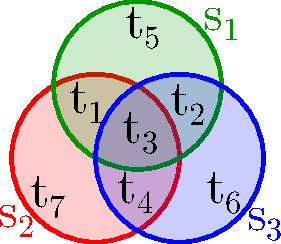
\includegraphics[width = 0.9\textwidth]{parity.pdf}
  \end{subfigure}\qquad
  \begin{subfigure}{0.2\textwidth}
    $(s1,s2,s3)=011 \Rightarrow$ error en $t4$
  \end{subfigure}
\end{figure}

\textbf{$\nota$} Recíprocamente si conozco $e$ la desigualdad me indica como son las distancias Hamming.

\textbf{$\propiedad$ Cota de Hamming(Cond. nec.):} 
Si un código de $M$ palabras clave de longitud $n$ corrige errores hasta orden $e$ $\Rightarrow$
$$
M \leq \frac{2^{n}}{\sum_{i=0}^{e}{n \choose i}} \ 
^{M: \#\text{palabras clave}, \quad e:\text{orden errores}}_{n: \#\text{dígitos(long. de palabra clave(dim. espacio))}}
$$

\textbf{$\definir$ Código de Hamming:} Detecta y corrige hasta errores simples.
$$
\operatorname{Hamming}(a, b), 
^{a\text{: \# dígitos}}_{b\text{: \# bits de mensaje}}
\
^{a-b\text{: \# bits de paridad}}
$$

\textbf{$\definir$ Síndrome o corrector:} Con un mensaje transmitido $t$, un error $e$ y matriz de paridad $A$, el síndrome $s$:
$$
s=A y=A(t+e)=A e,\quad \operatorname{size}(A) = (a-b) \times a
$$

\textbf{$\definir$ Palabras clave:} 
$$\mathbf{t}:A\mathbf{t}=\mathbf{0},\ \operatorname{Hamming}(a,b) \Rightarrow 2^b \text{palabras clave}$$

\textbf{$\definir$ Caso Hamming(7,4):}
$$
\boldsymbol{t}^{i}=\left(\begin{array}{c}
  t_{1}^{i} \\
  t_{2}^{i} \\
  t_{3}^{i} \\
  t_{4}^{i} \\
  t_{5}^{i} \\
  t_{6}^{i} \\
  t_{7}^{i}
\end{array}\right), \ \
\begin{aligned}
  t_{1}^{i}=x_{1}^{i},\quad t_{2}^{i}=x_{2}^{i} \\
  t_{3}^{i}=x_{3}^{i},\quad t_{4}^{i}=x_{4}^{i} \\
  t_{5}^{i}=x_{1}^{i} \oplus x_{2}^{i} \oplus x_{3}^{i} \\
  t_{6}^{i}=x_{2}^{i} \oplus x_{3}^{i} \oplus x_{4}^{i} \\
  t_{7}^{i}=x_{1}^{i} \oplus x_{3}^{i} \oplus x_{4}^{i}
\end{aligned}, \ \
\begin{aligned}
  \vec{t^i}: & i\text{-ésimo mensaje} \\
  &\text{ transmitido},\\
  &a \times 1 (1^os \ b \text{ dígitos}\\
  & \text{son el mensaje})\\
  \oplus: & \text{suma xor} (\oplus_2)
\end{aligned}
$$

\textbf{$\propiedad$ Tabla de decodificación:} Para $\operatorname{Hamming}(a,b)$, $r=a-b$.
$$
\begin{array}{c|c}
\text { Síndrome } & \text { Error } \\
\hline \underbrace{0\ldots0}_b & \underbrace{0\ldots0}_a \\
\hline A^T & I_a \\
\hline ^\text{síndromes}_\text{restantes} & ^\text{respectivos}_\text{errores} \\
\end{array}
\qquad \ejemplo \text{Ej.}: 
\begin{array}{c|c}
\text { Síndrome } & \text { Error } \\
\hline 000 & 00000 \\
\hline 101 & 10000 \\
010 & 01000 \\
011 & 00100 \\
111 & 00010 \\
100 & 00001 \\
\hline 110 & 01001 \\
001 & 01100
\end{array}
$$

\textbf{$\nota$ } Arrancas con los $\mathbf{s}$ y buscas sus respectivos $\mathbf{e}$

\textbf{$\propiedad$ Corregir errores:} La matriz de chequeo de paridad $A$ corrige errores de orden hasta $e$ $\Leftrightarrow$ todo conjunto de $2e$ columnas de $A$ es linealmente independiente.

\textbf{$\propiedad$ Dígitos de chequeo de paridad(cond. suf.):} El número $\ell$ de dígitos de chequeo de paridad debe cumplir
$$
2^{\ell}>\sum_{i=0}^{2 e-1} {n-1 \choose i}
$$

\textbf{$\propiedad$ Construir matriz chequeo de paridad:} 
Conociendo las dimensiones. Creo tantas columnas L.I. como bits de paridad. Luego creo columnas restantes como suma de las columnas anteriores 

\section{Clase 9:}

\textbf{$\definir$ Entropía diferencial conjunta:} 
La entropía diferencial conjunta asociada a una densidad conjunta $\rho\left(x_{1}, \ldots, x_{n}\right)$:
$$
\begin{aligned}
  &h\left(X_{1}, \ldots, X_{n}\right)=-\int \rho\left(x_{1}, \ldots, x_{n}\right) \log \left[\rho\left(x_{1}, \ldots, x_{n}\right)\right] \mathrm{d} x_{1} \ldots \mathrm{d} x_{n} \\
  &h(\boldsymbol{X})=-\int \rho(\boldsymbol{x}) \log [\rho(\boldsymbol{x})] \mathrm{d} \boldsymbol{x}
, \ \boldsymbol{x}=\left(x_{1}, \ldots, x_{n}\right)
\end{aligned}
$$

\textbf{$\propiedad$ Change variable:} $y=g(x)$
$$
\begin{aligned}
  f_{Y}(y)&=\frac{d F_{Y}(y)}{d y} =f_{X}\left(g^{-1}(y)\right)\left|\frac{d g^{-1}(y)}{d y}\right|=f_{X}(x)\left|\frac{d x}{d y}\right| \\
  h(Y) &=-\int f_{Y}(y) \log f_{Y}(y) d y \\
  &=-\int f_{Y}(y) \log f_{X}\left(g^{-1}(y)\right) d y-\int f_{Y}(y) \log \left|\frac{d x}{d y}\right| d y \\
  &=h(X)-\mathrm{E}\left[\log \left|\frac{d x}{d y}\right|\right]
\end{aligned}
$$

\textbf{$\definir$ Entropía diferencial condicionada:} 
La entropía diferencial condicionada de un conjunto de variables $\boldsymbol{X} =\left(X_{1}, \ldots, X_{n}\right)$ condicionadas a los valores que toma otro grupo de variables $\boldsymbol{Y}=\left(Y_{1}, \ldots, Y_{m}\right)$ vale
$$
h(\boldsymbol{X} \mid \boldsymbol{Y})=-\int \rho(\boldsymbol{x}, \boldsymbol{y}) \log [\rho(\boldsymbol{x} \mid \boldsymbol{y})] \mathrm{d} \boldsymbol{x} \mathrm{d} \boldsymbol{y}
$$

\textbf{$\propiedad$}
$
\begin{aligned}
  h(\boldsymbol{X}, \boldsymbol{Y})&=h(\boldsymbol{X})+h(\boldsymbol{Y} \mid \boldsymbol{X}) \\
  &=h(\boldsymbol{Y})+h(\boldsymbol{X} \mid \boldsymbol{Y})
\end{aligned}
$

\textbf{$\definir$ Kullback-Leibler:} 
Dadas dos densidades de prob. conjuntas $\rho_{1}(\boldsymbol{x})$ y $\rho_{2}(\boldsymbol{x})$ definidas sobre una variable aleatoria multivariada $\boldsymbol{X}=\left(X_{1}, \ldots, X_{n}\right),$ la divergencia de Kullback-Leibler entre ellas es
$$
D_{\mathrm{KL}}\left(\rho_{1} \| \rho_{2}\right)=\int \rho_{1}(\boldsymbol{x}) \log \left[\frac{\rho_{1}(\boldsymbol{x})}{\rho_{2}(\boldsymbol{x})}\right] \mathrm{d} \boldsymbol{x}
$$

\textbf{$\definir$ Información mutua:} 
Dadas las variables aleatorias continuas multivariadas $\boldsymbol{X}$ e $\boldsymbol{Y}$ con densidades conjuntas $\rho(\boldsymbol{x}, \boldsymbol{y}),$
la info. mutua $I(\boldsymbol{X} ; \boldsymbol{Y})$ vale
$$
\begin{aligned}
I(\boldsymbol{X} ; \boldsymbol{Y}) &=D_{\mathrm{KL}}[\rho(\boldsymbol{x}, \boldsymbol{y}) \| \rho(\boldsymbol{x}) \rho(\boldsymbol{y})] \\
&=h(\boldsymbol{x})-h(\boldsymbol{x} \mid \boldsymbol{y}) \\
&=h(\boldsymbol{y})-h(\boldsymbol{y} \mid \boldsymbol{x}) \\
&=h(\boldsymbol{x})+h(\boldsymbol{y})-h(\boldsymbol{x}, \boldsymbol{y})
\end{aligned}
$$
% $$
% I(X ; Y)=\sum_{x \in\{0,1\}} \sum_{y \in\{0,1\}} p(x, y) \log \left[\frac{p(x, y)}{p(x) p(y)}\right]
% $$
\begin{itemize}
  \item[$\bullet$] La $I$ no diverge
  \item[$\bullet$] $I$ y $D_{KL}$ pueden seguir interpretándose como el \# de preguntas ahorradas ($I$) o el \# de preguntas
  extras ($D_{KL}$).
  \item[$\bullet$] $0 \leq I$ y $0 \leq D_{KL}$ no están acotadas superiormente.
  \item[$\bullet$] No hay problema en calcular la $I$ entre una variable continua y otra discreta. 
  \item[$\bullet$] La $D_{KL}$ y $I$, permanecen inalteradas ante cambios de variables inyectivos del tipo $X^{\prime}=f(X), Y^{\prime}=g(Y).$
\end{itemize}
$$
\begin{aligned}
  {\tema} p(\mu)&=
  \left\{
    \begin{aligned}
      \frac{1}{\mu_{0}} & , \mu \in\left[\mu_{0}-\frac{\mu_0}{2}, \mu_{0}+\frac{\mu_0}{2}\right] \\
      0 & ,\text{c.o.c}
    \end{aligned}
  \right. \\
  h(\mu) &=\log \left(\mu_{0}\right)\\
  {\tema} p(\mu) &=\frac{\mathrm{e}^{-\mu / \mu_{0}}}{\mu_{0}} \\
  {\quad} h(\mu) &=1+\log \left(\mu_{0}\right)\\
  {\tema} p(\mu) &=\frac{2}{\pi \mu_{0}} \mathrm{e}^{-\mu^{2} / \pi \mu_{0}^{2}} \\
  {\quad} h(\mu) &=\frac{1}{2}+\log (\pi / 2)+\log \left(\mu_{0}\right) \\
  {\tema} p(\mu) &=\frac{k^{k}}{\Gamma(k) \mu_{0}^{k}} \mu^{k-1} \mathrm{e}^{-k \mu / \mu_{0}} \\ 
  h(\mu)&=k+\log \left(\mu_{0} / k\right)+\log [\Gamma(k)]+(1-k) \psi_{0}(k)
\end{aligned}
$$

% $$
% \begin{aligned}
% h_{\text {uniforme }} &=\log \left(\mu_{0}\right) \\
% h_{\text {exponencial }} &=1+\log \left(\mu_{0}\right) \\
% h_{\text {media Gaussiana }} &=\frac{1}{2}+\log (\pi / 2)+\log \left(\mu_{0}\right) \\
% h_{\text {gamma }} &=k+\log \left(\mu_{0} / k\right)+\log [\Gamma(k)]+(1-k) \psi_{0}(k),
% \end{aligned}
% $$

\section{Clase 10:}

\textbf{$\tema$ Técnica Maxentropy}

\begin{itemize}
  \item[$\bullet$] Listar todas las restricciones que queremos tener en cuenta.
  \item[$\bullet$] Construir el funcional $\mathcal{F}[P]$ del problema.
  \item[$\bullet$] Maximizar el funcional.
\end{itemize}

$\mathcal{F}[P(x)]$ es un funcional que depende de una función $P$, que a su vez depende de la variable
continua $x$. La dependencia es a través de una ecuación integral
$$
\begin{aligned}
  \mathcal{F}[P(x)]=&-\int_{-\infty}^{+\infty} P(x) \log [P(x)] \mathrm{d} x\\
  &+\sum_{j=1}^{n} \lambda_{j}\left[\int_{-\infty}^{+\infty} P(x) f(x) \mathrm{d} x-\alpha_{j}\right]
\end{aligned}
$$
el primer término es $h(x)$, y la $\sum$ contiene todas las restricciones, cada una con su multip. de Lagrange $\lambda_{j}$ y su valor fijado $\alpha_{j}$. Una de las restricciones (digamos la $i$-ésima) es de normalización($f_{i}(x)=1$, $\alpha_{i}=1$). 
$$ \left\lbrace
\begin{aligned}
  0 =& \frac{\partial \mathcal{F}[P(\mu)]}{\partial P\left(x^{*}\right)}=-1-\log \left[P\left(x^{*}\right)\right]+\sum_{j=1}^{n} \lambda_{j} f_{j}\left(x^{\star}\right) \\
  0 =& \int_{-\infty}^{+\infty} P(x) f_1(x) \mathrm{d} x-\alpha_{1} \\
  \qquad & \qquad \qquad \qquad \vdots \\
  0 =& \int_{-\infty}^{+\infty} P(x) f_n(x) \mathrm{d} x-\alpha_{n}
\end{aligned}
\right.
$$

\textbf{$\nota$}
Vemos que la derivada funcional puede calcularse derivando a lo bestia, considerando
que $P\left(x_{1}\right), P\left(x_{2}\right)$, etc., son las variables independientes de la función $\mathcal{F}[P(x)]$ e interpretando las
integrales como sumas.

\textbf{$\nota$}
Cuando todas las restricciones fijan el valor medio($\mu$) de determinadas funciones de la variable aleatoria (lo que equivale a decir que las restricciones son lineales en $P(\mu))$, Maxentropy arroja siempre exponencial en las funciones cuyo $\mu$ está fijado

\textbf{$\nota$} Se puede aplicar este mismo proceso en el discreto

\textbf{$\nota$} La distr. uniforme maximiza la $h(x)$ sin restricciones (más allá de la normalización).

\textbf{$\nota$} En variables $\in \mathbb{R}_0$, la distr. exponencial es la que maximiza la $h(x)$ cuando se fija el $\mu$.

\textbf{$\nota$} La distr. Gaussiana maximiza $h(x)$ cuando se fija la varianza(es irrelevante si se fija o no la media). Esta propiedad (junto al Teorema Central del Lim., cuando se puede suponer que su distr. proviene de la suma de diversos factores descorrelacionados), favorece a la distr. Gaussiana en procesos de los cuales solo conocemos el tamaño típico de las fluctuaciones.

\textbf{$\tema$ Canal gaussiano:} 
Sean $Y_{i}, X_{i}, Z_{i}$ variables aleatorias. $Y_{i}$ la salida, $X_{i}$ la entrada, $Z_{i}$ un ruido gaussiano y muestreado indepen. del tiempo y de los $X_j$.
$$
Y_{i}=X_{i}+Z_{i}
, \
\rho(z)=\frac{e^{-z^{2} / 2 N}}{\sqrt{2 \pi N}}, 
\rho(z): \text{Dens. de prob. de } z
$$
La magnitud $N$ de la varianza está fijada por el canal. Por cada valor $X_{i}$ que tengamos a la entrada, vamos a tener una Gaussiana de media $X_{i}$ y varianza $N$:
$$
\rho\left(y_{i} \mid x_{i}\right)=\frac{e^{-\left(y-x_{i}\right)^{2} / 2 N}}{\sqrt{2 \pi N}}
$$
Por esto, la capacidad del canal puede crecer con solo aumentar la separación entre símbolos de entrada. 

\textbf{$\ejemplo$} Imaginemos que trabajamos con un alfabeto $\mathcal{A}_{X}=\{\ldots,-2 \Delta,-\Delta, 0, \Delta, 2 \Delta, \ldots\}$. 

\begin{figure}[!ht]
  % \centering
  \begin{subfigure}{0.2\textwidth}
    \centering
    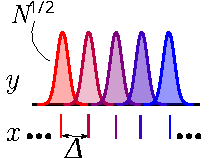
\includegraphics[width = 0.9\textwidth]{canalGaussiano.pdf}
  \end{subfigure}\qquad
  \begin{subfigure}{0.2\textwidth}
    La salida podemos obtener cualquier valor de $y$. Sin embargo, la superposición entre Gaussianas puede
    achicarse tanto como queramos, separando las entradas. 
  \end{subfigure}
\end{figure}
Cuando $\Delta \gg \sqrt{N}$ podemos
decodificar la entrada con mucha precisión. 
Si elegimos $\operatorname{los} X_{i}$ de entrada con distr. uniforme, la info. transmitida $\rightarrow \infty$ cuando $\Delta \rightarrow \infty$. 
la solución con capacidad ($C\rightarrow \infty$), presupone que podemos usar 4 señales de entrada arbitrariamente grandes, no es posbile. Se trata de maximizar la capacidad restringiendo la potencia (es decir, la varianza) de las $X$ a la entrada. 

\textbf{$\propiedad$ Estrategia 1:}
en vez de $\infty$ entradas discretas, tan solo un número finito, por
ejemplo 2. Para separar máximamente las entradas y aún cumplir con la restricción sobre la varianza, proponemos que $X$ pueda valer solo $\pm \sqrt{P}$, es decir.
$$
\rho(x)=\frac{1}{2} \delta(x-\sqrt{P})+\frac{1}{2} \delta(x+\sqrt{P})
$$
Esta es una posible estrategia. De hecho, es la mejor estrategia que podemos tomar si nuestro objetivo
es minimizar el error de decodificación. Sin embargo, se paga el costo de reducir drásticamente la entropía $H(X):$ del continuo de valores posibles que inicialmente teníamos para $X$, elegimos usar solo
dos. Agregar más entradas aumenta $H(X)$, pero también $H(X \mid Y)$.

\textbf{$\propiedad$ Estrategia 2:}
Conviene maximizar $I(X ; Y)$, que es lo que hacemos a continuación. Es decir, buscamos una distr. de entrada $\rho(x)$-sin pérdida de generalidad, podemos suponer que tiene media nula-que
maximice la info. transmitida por el canal, sujeta a la restricción
$$
\left\langle X^{2}\right\rangle=\int_{-\infty}^{+\infty} \rho(x) x^{2} \mathrm{~d} x \leq P
$$
para una constante conocida $P$, que representa la potencia de entrada que estamos dispuestos a costear.
La $I$ entre la entrada y la salida vale
$$
\begin{aligned}
I(X ; Y) &=h(Y)-h(Y \mid X) =h(Y)-h(X+Z \mid X) \\
&=h(Y)-h(Z \mid X) =h(Y)-h(Z) \\
&=h(Y)-\frac{1}{2} \ln (2 \pi e N) .
\end{aligned}
$$

\textbf{$\nota$}
$h(X+Z \mid X)=h(Z \mid X)$, por ser $X$ fijo.

\textbf{$\nota$}
$h(Z \mid X)=h(Z)$ porque $X,Z$ son independientes.

\textbf{$\nota$ Entropía diferencial de una gaussiana:} 
$h(Z)=\ln (2 \pi e N) / 2$

Como $h(Z)$ está fijada por el canal, maximizar la $I$ sujeta a potencia de entrada $P$ a maximizar la $h(Y)$ sujeta a potencia $P$. $$
\begin{aligned}
\left\langle Y^{2}\right\rangle &=\left\langle(X+Z)^{2}\right\rangle &=&\left\langle X^{2}\right)+2\langle X Z\rangle+\left\langle Z^{2}\right\rangle \\
&=\left\langle X^{2}\right\rangle+\left\langle Z^{2}\right\rangle&=&\left\langle X^{2}\right\rangle+N
\end{aligned}
$$
asi, la condición $\left(X^{2}\right\rangle \leq P$ $\Rightarrow$
$
\left\langle Y^{2}\right\rangle \leq P+N
$. Hay que encontrar una distr. de entrada $\rho(x)$ que maximice la $h(Y)$ sujeta a la restricción de la ecuación anterior. Usando Maxentropy, se tiene que la distr. $\rho(y)$ es:
$$\rho(y)=\frac{e^{-y^{2} / 2(P+N)}}{\sqrt{2 \pi(P+N)}}$$

Por la forma de $\rho(y)$:
$$
  \rho(x) =\frac{e^{-x^{2} / 2 P}}{\sqrt{2 \pi P}} ,\quad \rho(y \mid x) =\frac{e^{-(y-x)^{2} / 2 N}}{\sqrt{2 \pi N}}
$$
$\rho(x)$ muestrea valores cerca de 0 $\Rightarrow$ habrá confusiones a la salida. Pero si la varianza de entrada está fija, al elegir una Gaussiana es más lo que ganamos en $h(X)$ que lo que perdemos en $h(X \mid Y)$.

Con estas densidades $I$ es máxima $\therefore C = I$:
$$
\begin{aligned}
C &=h(Y)-h(Y \mid X) =\frac{1}{2} \ln [2 \pi e(P+N)]-\frac{1}{2} \ln [2 \pi e N] \\
&=\frac{1}{2} \ln \left(1+\frac{P}{N}\right), \quad 
\left({P \over N} 
  \text{ es un cociente } {\text{señal} \over \text{ruido}}\right)
\end{aligned}
$$

\section{Clase 11:}

\textbf{$\definir$ Estimadores:} 
Dada una variable aleatoria $X$
de alfabeto $\mathcal{A}_{X}$
con distr. de prob.
$P(x \mid \vartheta)$ que depende de un parámetro $\vartheta \in \Theta$ y un conjunto de muestras independientes $X_{1}, \ldots, X_{M}$ un estimador de $\vartheta$ es una función $\hat{\vartheta}: \mathcal{A}_{X}^{M} \rightarrow \Theta$.

\textbf{$\definir$ Estimador consistente:} 
Un estimador $\hat{\vartheta}$ es consistente si $n \rightarrow \infty, \hat{\vartheta}\left(X_{1}, \ldots, X_{n}\right) \rightarrow \vartheta$ (limite variables aleatorias). 

\textbf{$\definir$ Sesgo:} 
El sesgo $B(\vartheta)$ de un estimador es el error promedio que produce, donde el promedio se calcula para $\vartheta$ fijo. Es decir,
$$
B(\vartheta)= \langle \hat{\vartheta} \rangle -\vartheta=\int \mathrm{d}^{n} x p\left(x_{1}, \ldots, x_{n} \mid \vartheta\right) \hat{\vartheta}\left(x_{1}, \ldots, x_{n}\right) - \vartheta
$$
Un estimador es no sesgado si $B(\vartheta)=0, \forall \vartheta$

\textbf{$\nota$} Como vemos la notación $bias(\hat{\theta}) \neq B(\vartheta)$. Pero se refieren a lo mismo

\textbf{$\definir$ Error cuadrático medio(MSE) estimador:} 
$$\mathbb{E} \left[(\hat{\theta}-\theta)^{2}\right]$$
\textbf{$\propiedad$ Error MSE:} 
$$
\begin{aligned}
\mathbb{E} \left[(\hat{\theta}-\theta)^{2}\right] &=\mathbb{E} \left[\left(\hat{\theta}-\mathbb{E}  \hat{\theta}+\mathbb{E}  \hat{\theta}-\theta\right)^{2}\right] \\
&=\mathbb{E} \left[\left(\hat{\theta}-\mathbb{E}  \hat{\theta}\right)^{2}\right] 
+
\left[\mathbb{E} (\hat{\theta})-\theta\right]^{2} \\
&+ 2\left[\mathbb{E} (\hat{\theta})-\theta\right] \mathbb{E} \left[\hat{\theta}-\mathbb{E}  \hat{\theta}\right] \\
&=\operatorname{var}_{\theta}(\hat{\theta})+\operatorname{bias}^{2}(\hat{\theta}), \quad \operatorname{bias}(\hat{\theta})= \mathbb{E} (\hat{\theta})-\theta
\end{aligned}
$$

\textbf{$\definir$ Información de Fisher:} 
Denotada $J(\vartheta)$ asociada a una distr. de prob. $p(x \mid \vartheta)$ es la varianza
del puntaje. Es decir,
$$
\begin{aligned}
J(\vartheta) &=\left\langle(V-(V\rangle)^{2}\right\rangle =\left\langle V^{2}\right\rangle \\
&=\int_{-\infty}^{+\infty} p(x \mid \vartheta)\left[\frac{\partial}{\partial \vartheta} \ln p(x \mid \vartheta)\right]^{2} \mathrm{~d} x
\end{aligned}
$$
$$
J(\vartheta)=\left\langle\left(\frac{\partial}{\partial \vartheta} \ln P\left(x_{1}, \ldots, x_{n} \mid \vartheta\right)\right)^{2}\right\rangle
$$
$y$ los corchetes  $\langle \rangle$ denotan promedio pesado con la distr. $P\left(x_{1}, \ldots, x_{n} \mid \vartheta\right)$.

\textbf{$\propiedad$ Forma alternativa:} 
$$
\begin{aligned}
J(\vartheta) &=-\left\langle\frac{\partial^{2}}{\partial \vartheta^{2}} \ln [p(x \mid \vartheta)]\right\rangle \\
&=-\int_{-\infty}^{+\infty} p(x \mid \vartheta) \frac{\partial^{2}}{\partial \vartheta^{2}} \ln p(x \mid \vartheta) \mathrm{d} x
\end{aligned}
$$

\textbf{$\definir$ Error cuadrático medio:}
$$
E^{2}(\vartheta) = E[ \hat{\vartheta} - \vartheta ] = \int_{-\infty}^\infty p\left(x_{1}, \ldots, x_{n} \mid \vartheta\right)\left[\hat{\vartheta}\left(x_{1}, \ldots, x_{n}\right)-\vartheta\right]^{2} {d}^{n} x 
$$

\textbf{$\definir$ Cota de Crámer-Rao:}
$$
\begin{aligned}
  &\qquad \qquad \qquad E^{2}(\vartheta) J(\vartheta) \geq 1 \\
  &\left\{\int_{-\infty}^{+\infty} p(x \mid \vec{\vartheta})[\hat{\vartheta}(x)-\vartheta]^{2} \mathrm{~d} x\right\}
  \cdot \\
  &\left\{\int_{-\infty}^{+\infty} p(x \mid \vartheta)\left[\frac{\partial}{\partial \vartheta} \ln p(x \mid \vartheta)\right]^{2} \mathrm{~d} x\right\} \geq 1  
\end{aligned}
$$

\textbf{$\definir$ Eficiente:} 
Un estimador $\hat{\theta}$ es eficiente si su MSE es pequeño, (según la Cota de Crámer Rao):
$$
E^{2}(\vartheta) J(\vartheta) \geq 1,
$$

\textbf{$\definir$ Puntaje:} 
El puntaje de una variable aleatoria $X$ muestreada con prob. $p(x \mid \vartheta)$ es una nueva variable
aleatoria $V$ que se obtiene de transformar $X$ con la función
$$
V=\frac{\partial}{\partial \vartheta} \ln [p(X \mid \vartheta)]
$$
% Cada valor muestreado de
% la variable aleatoria $X$ debe ser procesada con la fórmula así obtenida, $y$ producir una variable aleatoria
% $V$.

\textbf{$\nota$}
$p(x \mid \vartheta)$ debe ser derivable (y $\boldsymbol{\therefore}$, continua) en $\vartheta$, salvo un número finito de puntos, pero, puede no ser continua en $x$. $X$ puede ser una variable discreta, $p(x \mid \vartheta)$ puede solo estar definida en un número finito de $x's$, una suma de $\delta$.

\textbf{$\propiedad$ Valor medio del puntaje:} 
$\langle V \rangle = 0$

\textbf{$\propiedad$ No negatividad:} 
$J(\vartheta) \geq 0$ 

\textbf{$\propiedad$ Aditividad:} 
Si $\left(X_{1}, \ldots, X_{n}\right)$ son $n$ muestras indepen. de $p(x \mid \vartheta)$ $\Rightarrow$ $J_{n}(\vartheta)$:
$$
J_{n}(\vartheta)=n J_{1}(\vartheta), 
\begin{aligned}
  J_{n} \text{usa } p\left(x_{1}, \ldots, x_{n} \mid \vartheta\right) \\
  J_{1} \text{usa } p\left(x_{1}, \ldots, x_{n} \mid \vartheta\right)
\end{aligned}
$$

\textbf{$\propiedad$ Cambio de variable:} 
$$
\begin{aligned}
I^{\theta}(\theta) &=I^{\eta}(\eta)\left(J_{\theta}^{\eta}\right)^{2} \\
I^{\theta}(\theta) &=I^{\eta}(\eta)\left( \frac{\partial \eta}{\partial \theta} \right)^{2} (\text{1D})
\end{aligned}
$$

\textbf{$\ejemplo$ Binomial:} $\vartheta$ es la prob. de éxito:
$$
\begin{aligned}
  P(k \mid \vartheta)
  &=\frac{N !}{k !(N-k) !} \vartheta^{k}(1-\vartheta)^{N-k} , N \in \mathbb{N} ^\text{\# of trials}_{(parameter)}\\
  &, k \in\{0,1, \ldots, n\}, ^\text{\# of successes}_{(variable)}
\end{aligned}
$$
$$
\begin{aligned}
    \mathrm{E}(X) 
    &= \sum_{k=0}^{n} k {n \choose k} p^{k} q^{n-k} = \sum_{k=1}^{n} k {n \choose k} p^{k} q^{n-k} \\
    &= \sum_{k=1}^{n} n {n-1 \choose k-1} p^{k} q^{n-k} 
    \left( 
        k {n \choose k} =n {n-1 \choose k-1} 
    \right) 
    \\
    &=n p \sum_{k=1}^{n}{n-1 \choose k-1} p^{k-1} q^{(n-1)-(k-1)} 
    \\ &
    \left( 
        \text {sacar } n p \text { y }
        (n-1)-(k-1)=n-k
    \right) 
    \\
    &=n p \sum_{j=0}^{m} {m \choose j} p^{j} q^{m-j}
    \left( 
        \text{putting } 
        ^{m=n-1}_{j=k-1}
    \right) 
    \\
    &=n p \left( \text { Binomial Theorem and } p+q=1 \right) 
\end{aligned}
$$
El puntaje vale
$$
\begin{aligned}
V(K) &=\frac{\partial}{\partial \theta} \ln [P(K \mid v)] \\
&=\frac{\partial}{\partial \theta}\{\ln (N !)-\ln (K !)-\ln [(N-K) !] \\
&+k \ln (\vartheta)+(N-K) \ln (1-\vartheta)\} \\
&=\frac{K}{\vartheta}-\frac{N-K}{1-\vartheta}=\frac{K-N \vartheta}{\partial(1-\vartheta)}
\end{aligned}
$$
Dado que $\langle K\rangle=N \vartheta$, en este ejemplo, $V$ es proporcional a $K-\langle K\rangle$. Por esto el valor medio $=0$.
$$\text{Informacion fisher: }J(\vartheta)=\frac{N}{\vartheta(1-\vartheta)}$$

\textbf{$\ejemplo$ Exponencial:} 
$$
^\text{parametrizada con un} 
_{\text{tiempo de vida medio }\vartheta_{1}} : 
p\left(x \mid \partial_{1}\right)=\frac{e^{-x / \theta_{1}}}{\vartheta_{1}}
$$
El puntaje vale
$$
\begin{aligned}
V &=\frac{\partial}{\partial \vartheta_{1}} \ln \left[p\left(X \mid \vartheta_{1}\right)\right] &= &\frac{\partial}{\partial \vartheta_{1}}\left[-\frac{X}{\partial_{1}}-\ln \left(\partial_{1}\right)\right] \\
&=\frac{X}{\vartheta_{1}^{2}}-\frac{1}{\vartheta_{1}} &= &\frac{X-\vartheta_{1}}{\vartheta_{1}^{2}}
\end{aligned}
$$
Nuevamente obtuvimos $V \propto X-\langle X\rangle$. Por esto el valor medio se anula.
$$\text{Información Fisher: }J\left(\vartheta_{1}\right)=\frac{1}{\vartheta_{1}^{2}}$$

\textbf{$\ejemplo$ Exponencial:} 
$$
\text{Con una tasa media } \vartheta_{2} :
p\left(x \mid \vartheta_{2}\right)=\vartheta_{2} \mathrm{e}^{-\theta_{2} x}
$$
El puntaje vale
$$
\begin{aligned}
V &=\frac{\partial}{\partial \vartheta_{2}} \ln \left[p\left(X \mid \vartheta_{2}\right)\right] =\frac{\partial}{\partial \vartheta_{2}}\left[-\vartheta_{2} X+\ln \left(\vartheta_{2}\right)\right] \\
&=-X+\frac{1}{\vartheta_{2}}
\end{aligned}
$$
Una vez más, obtuvimos $V \propto X-\langle X\rangle$, con una constante de proporcionalidad negativa.
$$\text{Informacion fisher: }J\left(\vartheta_{2}\right)=\frac{1}{\vartheta_{2}^{2}}$$

\textbf{$\definir$ La información de Fisher como expresión local de la divergencia de Kullback-Leibler:}
$$
\begin{aligned}
  &D_{\mathrm{KL}}[p(x \mid \vartheta+\mathrm{d} \vartheta) \| p(x \mid \vartheta)] \approx  \frac{(\mathrm{d} \vartheta)^{2}}{2} J(\vartheta)\\
  &D_{\mathrm{KL}}[p(x \mid \vartheta \| p(x \mid \vartheta+\mathrm{d} \vartheta))] \approx \frac{(\mathrm{d} \vartheta)^{2}}{2} \cdot J(\vartheta)
\end{aligned}
$$

\textbf{$\tema$ Repaso de tensores métricos:} 
Un tensor métrico $M$ debe ser simétrico y definido positivo
(todos sus autovalores positivos), define un producto escalar
$$
\left\langle\boldsymbol{v}^{\alpha}, \boldsymbol{v}^{b}\right\rangle=\left(\boldsymbol{v}^{a}\right)^{t} M \boldsymbol{v}^{b},
$$
donde $t$ representa "traspuesto". Las dist. y angulos
$$
\begin{aligned}
d\left(\boldsymbol{v}^{\alpha}, \boldsymbol{v}^{b}\right) &=\left|\boldsymbol{v}^{a}-\boldsymbol{v}^{6}\right|, \ |\boldsymbol{v}| =\sqrt{\langle\boldsymbol{v}, \boldsymbol{v}\rangle} \\
\alpha\left(\boldsymbol{v}^{\alpha}, \boldsymbol{v}^{b}\right) &=\operatorname{arccos}\left(
  \frac{
    \left\langle
    \boldsymbol{v}^{a}, \boldsymbol{v}^{b}
    \right\rangle
    }{\left|\boldsymbol{v}^{a}\right|\left|\mathbf{v}^{b}\right|}
  \right)
\end{aligned}
$$

\textbf{$\definir$ Información de Fisher, parámetro multidimensional:}
Si $\vartheta$ proviene de un espacio de parámetros $\Theta$ de dimensión $n$, la información de
Fisher $J(\boldsymbol{\vartheta})$ es un tensor de rango 2 de dimensión $n \times n$ cuyas componentes valen
$$
\begin{aligned}
J(\boldsymbol{\vartheta})_{k \ell} &=\left\langle\frac{\partial \ln [p(x \mid \boldsymbol{\vartheta})]}{\partial \boldsymbol{\vartheta}_{k}} \frac{\partial \ln [p(x \mid \boldsymbol{\vartheta})]}{\partial \vartheta_{k}}\right\rangle \\
&=-\left\langle\frac{\partial^{2} \ln [p(x \mid \boldsymbol{\vartheta})]}{\partial \boldsymbol{\vartheta}_{k} \partial \boldsymbol{\vartheta}_{k}}\right\rangle
\end{aligned}
$$
donde los valores medios se calculan pesados con la distr. $p(x \mid \vartheta)$. Para el continuo:
$$
\begin{aligned}
J_{k \ell} &=\int p(x \mid \vartheta)\left[\frac{\partial \ln [p(x \mid \vartheta)]}{\partial v_{k}}\right]\left[\frac{\partial \ln [p(x \mid \vartheta)]}{\partial v_{\ell}}\right] \mathrm{d} x \\
&=-\int p(x \mid \boldsymbol{\vartheta})\left[\frac{\partial^{2} \ln [p(x \mid \boldsymbol{v})]}{\partial \vartheta_{k} \partial \vartheta_{\ell}}\right] \mathrm{d} x
\end{aligned}
$$
y con variables discretas, las integrales se reemplazan por sumas. 

\textbf{$\propiedad$ Propiedades del tensor $J(\mathbf{\vartheta})$:}
$$
\begin{aligned}  
   &\qquad\ {\tema} \text{Es simétrico, por definición.} \\
   &\qquad\ {\tema} \text{Es definido no negativo (autovalores no negativos)}
\end{aligned}
$$

\textbf{$\definir$ Cota de Crámer-Rao(Tensorial):} 
se transforma en una ecuación matricial
$$
E^{2}(\boldsymbol{\vartheta}) J(\boldsymbol{\vartheta}) \geq \mathbb{I}
$$
donde el error cuadrático medio $E(\boldsymbol{\theta})$ es una matriz de $n \times n$ de componentes
$$
E_{k \ell}^{2}=\left\langle 
\left(
  \hat{\vartheta}_{k}(X)-\vartheta_{k}
  \right)
\left(
  \hat{\nu}_{\ell}(X)-\vartheta_{\ell}
  \right)
  \right\rangle,
$$
$y$ la desigualdad $E J \geq \mathbb{I}$ significa que todos los autovalores de la matriz producto $E . J$ son $\geq 1$.

\textbf{$\definir$ La información de Fisher como expresión local de la divergencia de Kullback-Leibler(Tensorial):}
$$
D_{\mathrm{KL}}[p(x \mid \boldsymbol{\vartheta}+\mathrm{d} \boldsymbol{\vartheta}) \| p(x \mid \boldsymbol{\theta})] \approx \frac{1}{2} \mathrm{~d} \boldsymbol{\vartheta}^{t} J(\boldsymbol{\vartheta}) \mathrm{d} \boldsymbol{\vartheta}
$$
\textbf{$\propiedad$ Transformación:} 
Si el parámetro $\vartheta$ es transformado en un nuevo parámetro $\varphi=F(\vartheta)$, $\Rightarrow$ la $J(\boldsymbol{v})$ transforma como
$$
J(\boldsymbol{v})=C^{t} J(\varphi) C
, \
C_{k \ell}=\frac{\partial F_{k}}{\partial \vartheta_{\ell}} \
^\text{es la matriz jacobiana}
_\text{de la transformación}
$$

\textbf{$\propiedad$ Teorema de procesamiento de datos:}
Si transformamos la variable aleatoria $X$ en $Y=f(X) \Rightarrow$
$$
J_{X}(\boldsymbol{\vartheta}) \geq J_{Y}(\boldsymbol{\vartheta})
$$

\textbf{$\tema$ Tensor métrico:} $J_{ik}(\vartheta)$ Permite calcular dist. en el espacio de parámetros. Calculemos la dist.
entre los parámetros $\boldsymbol{\theta}^{a}=\left(\mu^{a}, \sigma^{a}\right)^{t}$ y $\boldsymbol{\theta}^{b}=\left(\mu^{b}, \sigma^{b}\right)^{t}$ 
$$
\begin{aligned}
\operatorname{Dist}\left(\boldsymbol{\vartheta}^{a}, \boldsymbol{\vartheta}^{b}\right) &=\int_{\text {Camino }}|\mathrm{d} \ell| \\
&=\int_{\text {Camino }} \sqrt{\mathrm{d} \boldsymbol{\vartheta}(t)^{T} J[\boldsymbol{\vartheta}(t)] \mathrm{d} \boldsymbol{\vartheta}(t)} \\
&=\int_{0}^{1} \sqrt{\dot{\boldsymbol{\vartheta}}^{t} J(\boldsymbol{\vartheta}) \dot{\boldsymbol{\vartheta}}} \mathrm{d} t
\end{aligned}
$$

\textbf{$\ejemplo$ Tensor métrico:} 
usando la métrica de Fisher de la distr.
Gaussiana. Conectamos los puntos a través de un camino lineal
$$
\boldsymbol{v}(t)=\left(\begin{array}{c}
\mu(t) \\
\sigma(t)
\end{array}\right)=\left(\begin{array}{c}
t \mu^{b}+(1-t) \mu^{a} \\
t \sigma^{b}+(1-t) \sigma^{a}
\end{array}\right)
$$

con $t \in[0,1]$. La dist. se calcula integrando diferenciales
de dist. $d\hat{\ell}$ a lo largo del camino, teniendo en cuenta que
$$
\mathrm{d} \ell=\mathrm{d} \boldsymbol{\vartheta}(t)=\dot{\boldsymbol{\vartheta}} \mathrm{d} \boldsymbol{t}=\left(\begin{array}{c}
\mu^{b}-\mu^{a} \\
\sigma^{b}-\sigma^{a}
\end{array}\right) \mathrm{d} t,
$$
donde $\dot{\vartheta}=\mathrm{d} \vartheta(t) / \mathrm{d} t$. La distancia es una cantidad siempre positiva. 
$$
\begin{aligned}
  \operatorname{Dist}\left(\boldsymbol{\vartheta}^{a}, \boldsymbol{\vartheta}^{b}\right) &=\frac{\sqrt{\left(\mu^{b}-\mu^{a}\right)^{2}+2\left(\sigma^{b}-\sigma^{2}\right)^{2}}}{\sigma^{b}-\sigma^{a}} \int_{0}^{\sigma^{b}-\sigma^{a}} \frac{\mathrm{d} z}{\sigma^{a}+z} \\
&=\frac{\sqrt{\left(\mu^{b}-\mu^{a}\right)^{2}+2\left(\sigma^{b}-\sigma^{2}\right)^{2}}}{\sigma^{b}-\sigma^{a}} \ln \left(\frac{\sigma^{b}}{\sigma^{a}}\right)
\end{aligned}
$$

\textbf{$\nota$} Si trasladamos $\mu^{a}$ y $\mu^{b}$ en una cantidad fija, la $Dist.$ no varía. Pero si desplazamos las $\sigma$, la $Dist.$ varia. De hecho, si alguna $\sigma \rightarrow 0 \Rightarrow$ $Dist. \rightarrow \infty$. Si alguna $\sigma \rightarrow 0$, la distr. correspondiente tiende a una $\delta$ Dirac.

\textbf{$\ejemplo$ Tensor:} 
de Fisher de $2 \times 2$ para la distr. Gaussiana
Dada la distr.
$$
p(x \mid \mu, \sigma)=\frac{e^{-(z-\mu)^{2} / 2 \sigma^{2}}}{\sqrt{2 \pi \sigma^{2}}}
$$
$$
\begin{aligned}
J(\mu, \sigma) &
=
\left(\begin{array}{ll}
J_{\mu \mu} & J_{\mu \sigma} \\
J_{\mu \sigma} & J_{\sigma \sigma}
\end{array}\right)
&
=
\frac{1}{\sigma^{2}}\left(\begin{array}{ll}
1 & 0 \\
0 & 2
\end{array}\right) .
\end{aligned}
$$

\end{document}
%
% ****** End of file apssamp.tex ******
